\documentclass[compress]{beamer}
\usepackage{ifthen,verbatim,ulem,hyperref}

\newcommand{\isnote}{}
\xdefinecolor{lightyellow}{rgb}{1.,1.,0.25}
\xdefinecolor{darkblue}{rgb}{0.1,0.1,0.7}

%% Uncomment this to get annotations
%% \def\notes{\addtocounter{page}{-1}
%%            \renewcommand{\isnote}{*}
%% 	   \beamertemplateshadingbackground{lightyellow}{white}
%%            \begin{frame}
%%            \frametitle{Notes for the previous page (page \insertpagenumber)}
%%            \itemize}
%% \def\endnotes{\enditemize
%% 	      \end{frame}
%%               \beamertemplateshadingbackground{white}{white}
%%               \renewcommand{\isnote}{}}

%% Uncomment this to not get annotations
\def\notes{\comment}
\def\endnotes{\endcomment}

\setbeamertemplate{navigation symbols}{}
\setbeamertemplate{headline}{\mbox{ } \hfill
\begin{minipage}{5.5 cm}
\vspace{-0.75 cm} \small
\end{minipage} \hfill
\begin{minipage}{4.5 cm}
\vspace{-0.75 cm} \small
\begin{flushright}
\ifthenelse{\equal{\insertpagenumber}{1}}{}{Jim Pivarski \hspace{0.2 cm} \insertpagenumber\isnote/\pageref{numpages}}
\end{flushright}
\end{minipage}\mbox{\hspace{0.2 cm}}\includegraphics[height=1 cm]{../cmslogo} \hspace{0.1 cm} \vspace{-1.05 cm}}

\begin{document}
\newcommand{\met}{$E_{\rm{T}}\hspace{-1.1em}/$\hspace{0.7em}}
\newcommand{\metv}{$\vec{E}_{\rm{T}}\hspace{-1.1em}/$\hspace{0.7em}}

\begin{frame}
\vfill
\begin{center}
\textcolor{darkblue}{\Large Early Discovery Channels in CMS}

\vfill
\begin{columns}
\column{0.5\linewidth}
\begin{center}
\large
\textcolor{darkblue}{Jim Pivarski}

\vspace{0.2 cm}
\scriptsize \textcolor{darkblue}{Texas A\&M University}
\end{center}
\end{columns}

\begin{columns}
\column{0.5\linewidth}
\begin{center}
\scriptsize
{\it on behalf of the Compact Muon Solenoid (CMS) collaboration}
\end{center}
\end{columns}

\vfill
LHCDM@MCTP: The LHC and Dark Matter

\vspace{0.2 cm}
 6 January, 2009

\end{center}
\end{frame}

%% \begin{notes}
%% \item This is the annotated version of my talk.
%% \item If you want the version that I am presenting, download the one
%% labeled ``slides'' on Indico (or just ignore these yellow pages).
%% \item The annotated version is provided for extra detail and a written
%% record of comments that I intend to make orally.
%% \item Yellow notes refer to the content on the {\it previous} page.
%% \item All other slides are identical for the two versions.
%% \end{notes}

\small

\begin{frame}
\frametitle{``Early discovery channels''}

\begin{columns}
\column{0.6\linewidth}

\vspace{-1 cm}
\begin{itemize}
\item Based on recent LHC schedules, we can hope for about
  100~pb$^{-1}$ of 10~TeV collisions in 2009
\item Full re-analysis at 10~TeV is \mbox{under study,\hspace{-0.5 cm}} but most production
  cross-sections will be reduced by about a factor of 2, depending on
  mass
\item In this talk: 14~TeV analyses reoptimized for 100~pb$^{-1}$
\begin{itemize}
\item new results, \mbox{post-Physics TDR\hspace{-1 cm}}
\item roughly what we may see \mbox{this year\hspace{-1 cm}}
\end{itemize}
\end{itemize}
\column{0.5\linewidth}

\vspace{0.5 cm}
\mbox{ } \hfill \hfill J.\ Stirling \hfill \mbox{ }

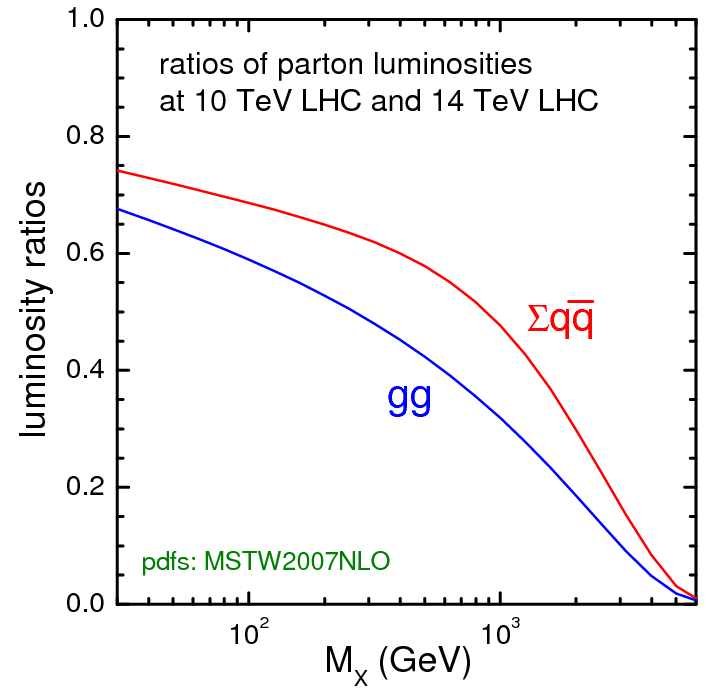
\includegraphics[width=\linewidth]{sterling_plot.png}
\end{columns}

\vspace{-0.6 cm}
\hspace{-0.83 cm} \textcolor{darkblue}{\Large Outline of this talk}

\vspace{-0.2 cm}
\begin{enumerate}\setlength{\itemsep}{-0.05 cm}
\item CMS detector
\item Standard Model: rediscovery, service measurements, and new modes
\item Brief note on SUSY
\item Di-object signature searches: $e^+e^-$, $\mu^+\mu^-$, jet-jet, jet-\met, \ldots
\item Heavy, long-lived particles and other models
\end{enumerate}
\end{frame}

\begin{frame}
\frametitle{CMS detector}
\begin{itemize}\setlength{\itemsep}{-0.05 cm}
\item Nearly $4\pi$ general-purpose detector
\item All-silicon tracker
\item Solenoidal magnetic field
\item Highly-redundant muon tracking system (44 muon layers in barrel)
\end{itemize}

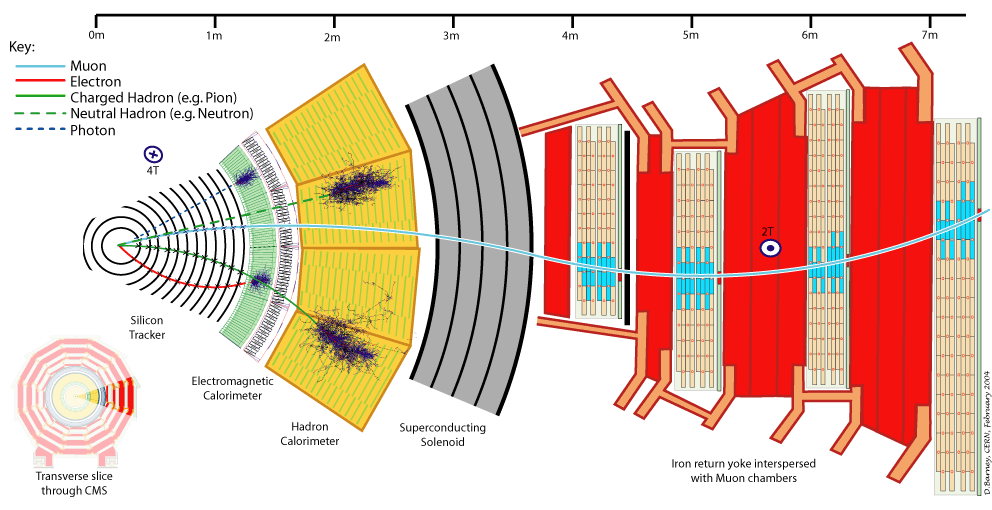
\includegraphics[width=\linewidth]{CMS_Slice.png}

\mbox{ }
\end{frame}

\begin{frame}
\frametitle{Rediscovering the Standard Model}

\begin{itemize}
\item Signals and backgrounds at \textcolor{red}{10~pb$^{-1}$}
\end{itemize}

\begin{tabular}{c c c}
& $e^\pm\nu$ or $e^+e^-$ & $\mu^\pm\nu$ or $\mu^+\mu^-$ \\

\includegraphics[height=2.7 cm]{wpm.png}\vspace{-0.05 cm} & 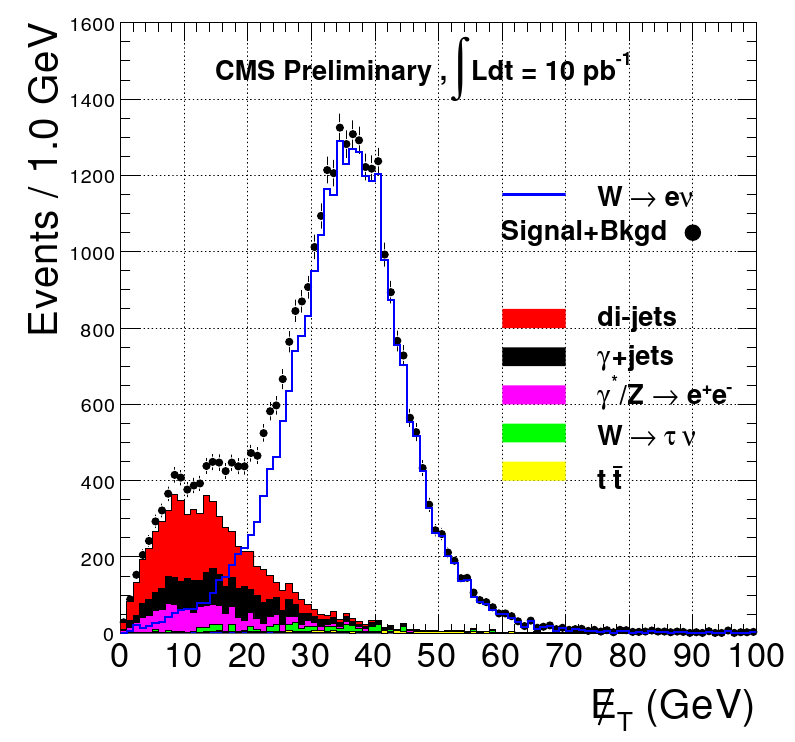
\includegraphics[height=2.7 cm]{W_ee_10pb-1.png}\vspace{-0.05 cm} & 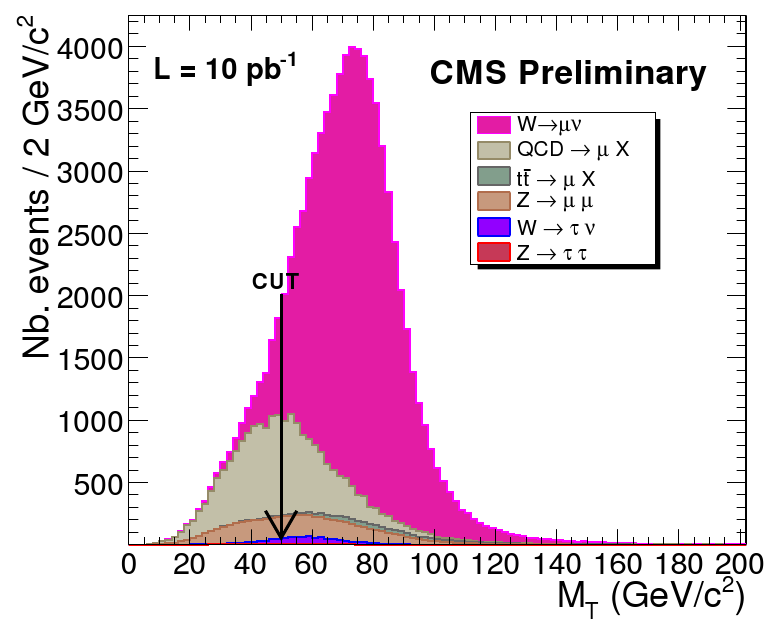
\includegraphics[height=2.7 cm]{W_mumu_10pb-1.png}\vspace{-0.05 cm} \\
& {\scriptsize missing transverse energy} & {\scriptsize transverse mass} \\
& & \\

\includegraphics[height=2.7 cm]{z0.png}\vspace{-0.05 cm}  & 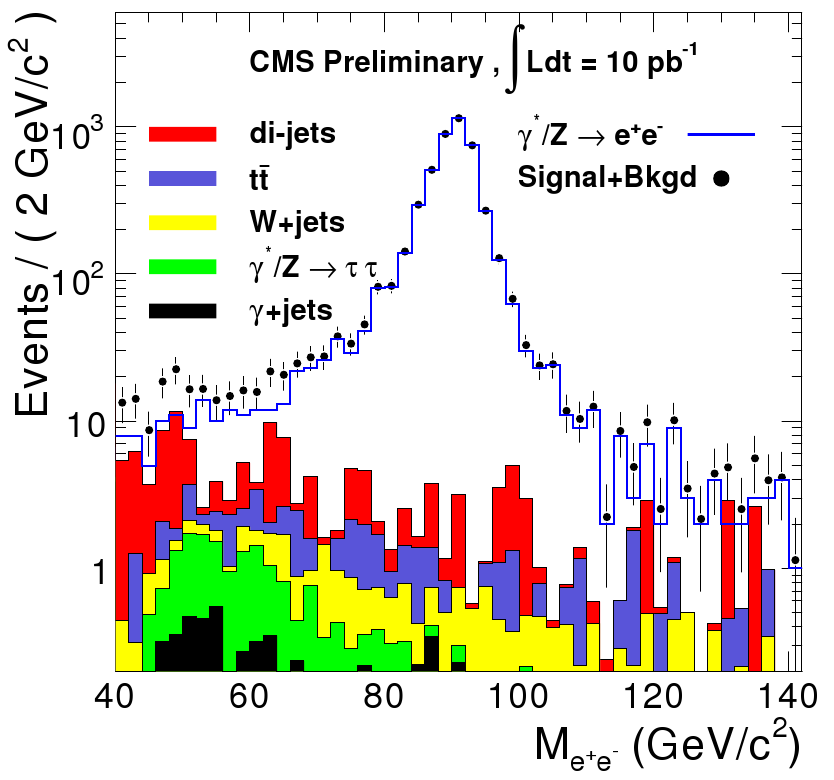
\includegraphics[height=2.7 cm]{Z_ee_10pb-1.png}\vspace{-0.05 cm} & 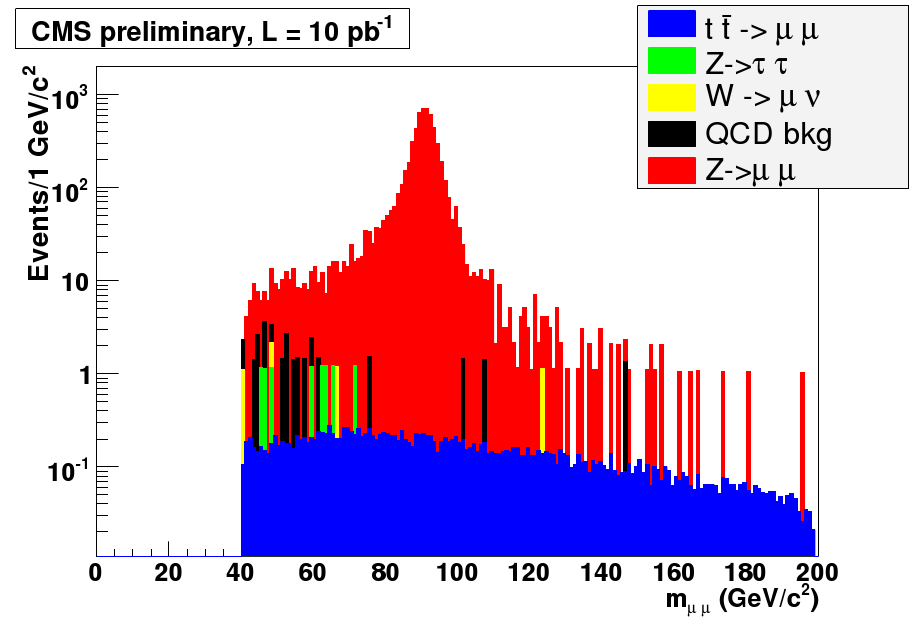
\includegraphics[height=2.7 cm]{Z_mumu_10pb-1.png}\vspace{-0.05 cm} \\
& {\scriptsize $e^+e^-$ mass} & {\scriptsize $\mu^+\mu^-$ mass} \\
\end{tabular}

\begin{itemize}
\item Top quarks observable with 10--100~pb$^{-1}$ (see Oliver's talk)
\end{itemize}
\label{rediscovering_standard_model}
\end{frame}

\begin{frame}
\frametitle{Using the SM for future discoveries}

\begin{columns}
\column{0.65\linewidth}
\begin{itemize}
\item Determine electron and muon efficiencies by tagging one leg of a $Z\to\ell\ell$, probing the other (right)

\item $W^\pm$ charge asymmetry (below)

\mbox{ } \hfill {\scriptsize $\displaystyle A(\eta) = \frac{(d\sigma/d\eta)(W^+) - (d\sigma/d\eta)(W^-)}{(d\sigma/d\eta)(W^+) + (d\sigma/d\eta)(W^-)}$} \hfill \mbox{ }

\begin{itemize}
\item probes $u$/$d$ PDFs for other analyses
\item depends only on detector \mbox{issues that are\hspace{-1 cm}} \mbox{currently being studied with real data in cosmic ray asymmetry\hspace{-5 cm}}
\end{itemize}
\end{itemize}

\column{0.35\linewidth}
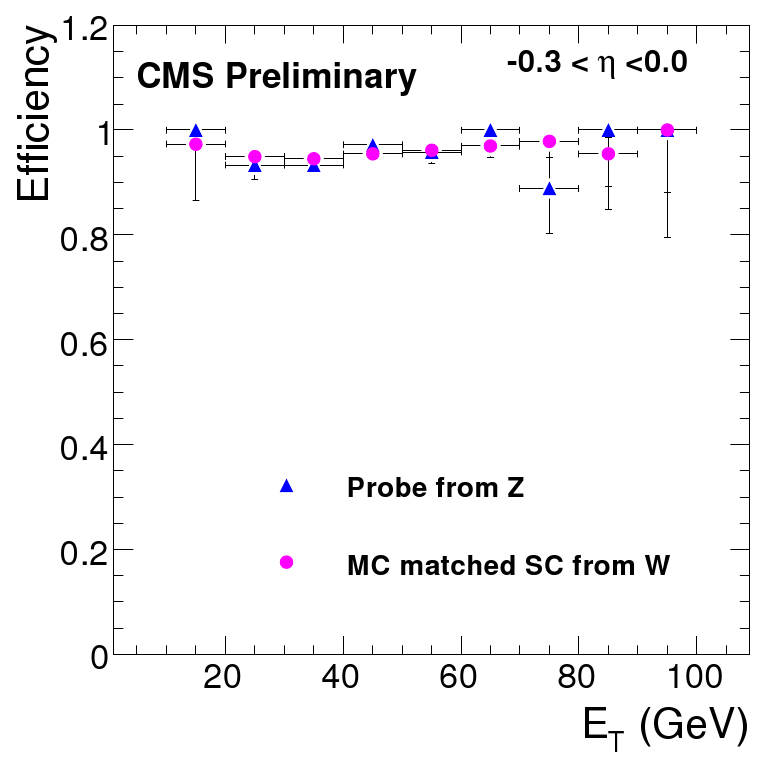
\includegraphics[width=\linewidth]{electroneff_tag-probe.png}
\end{columns}

\vfill
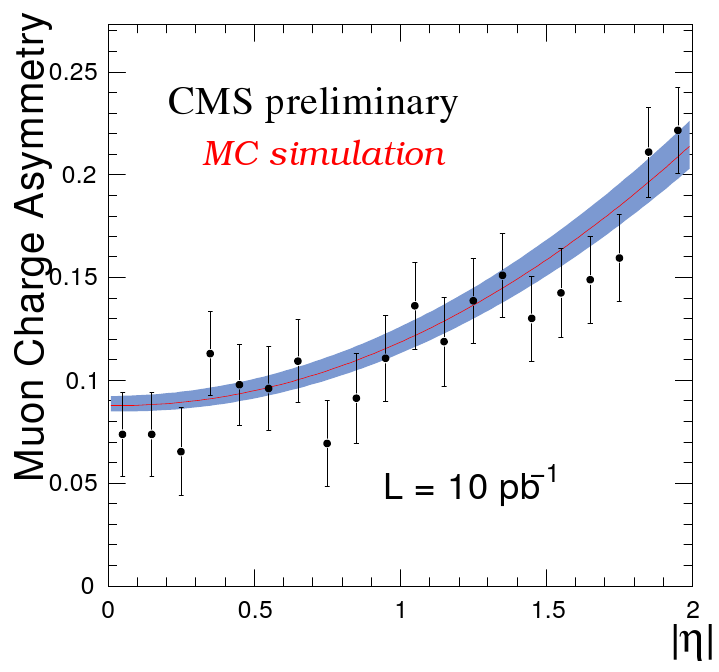
\includegraphics[width=0.35\linewidth]{W_chargeasymmetry_10pb-1.png}
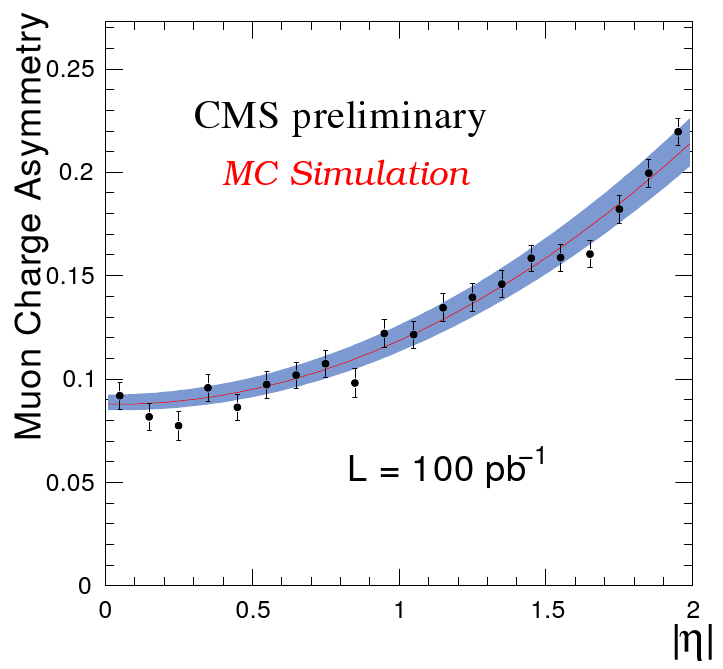
\includegraphics[width=0.35\linewidth]{W_chargeasymmetry_100pb-1.png}
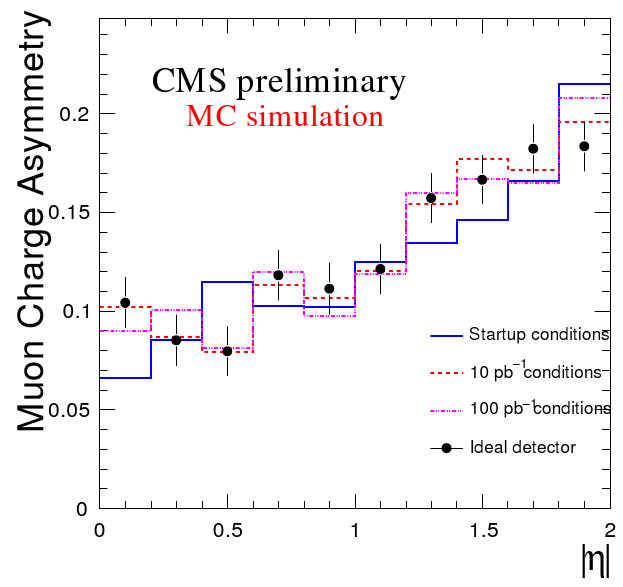
\includegraphics[width=0.35\linewidth]{W_chargeasymmetry_conditions.png}
%% 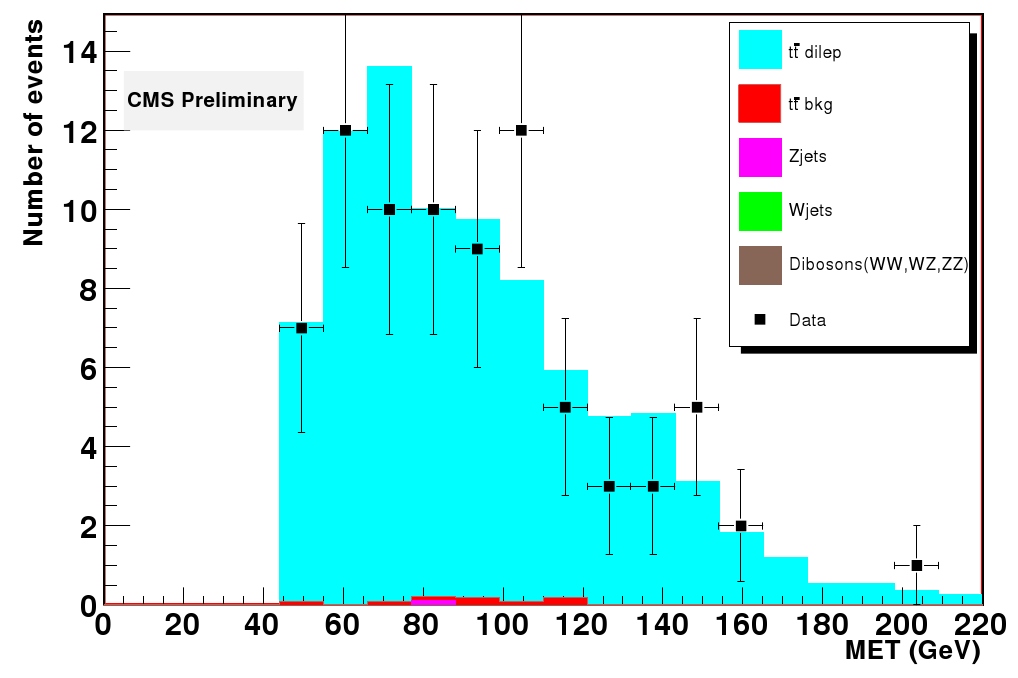
\includegraphics[width=0.25\linewidth]{ttbar_dilepton_100pb-1.png}
%% 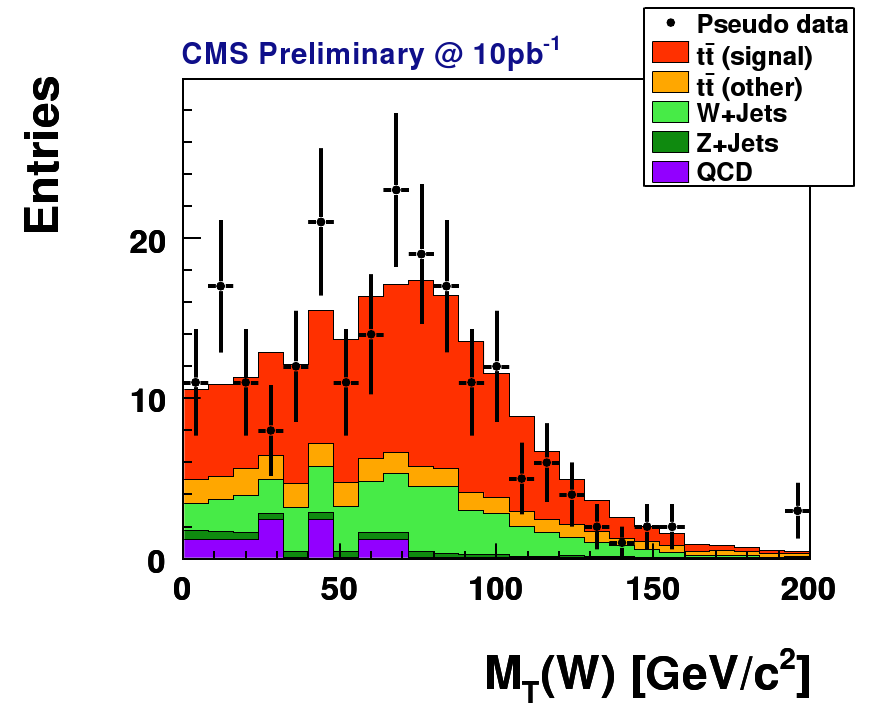
\includegraphics[width=0.25\linewidth]{ttbar_semileptonic_10pb-1.png}
\label{using_standard_model_for_future}
\end{frame}

\begin{frame}
\frametitle{Discoveries in the Standard Model}

\vfill
\begin{columns}
\column{0.6\linewidth}

\mbox{ } \hfill 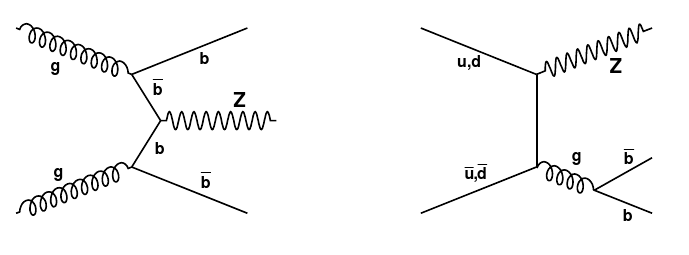
\includegraphics[width=0.65\linewidth]{Zbb_diagrams.png} \hfill \mbox{ }

\vspace{-0.25 cm}
\begin{itemize}
\item $Zb\bar{b}$ and \sout{di-bosons} (re-discovery):
\begin{itemize}
\item background for Higgs searches \\ $H \to Z Z \to 4\mu$, \mbox{SUSY $H \to 2\tau (\mu)$\hspace{-1 cm}}
\end{itemize}
\end{itemize}

\vspace{0.8 cm}
\mbox{ }

\column{0.4\linewidth}
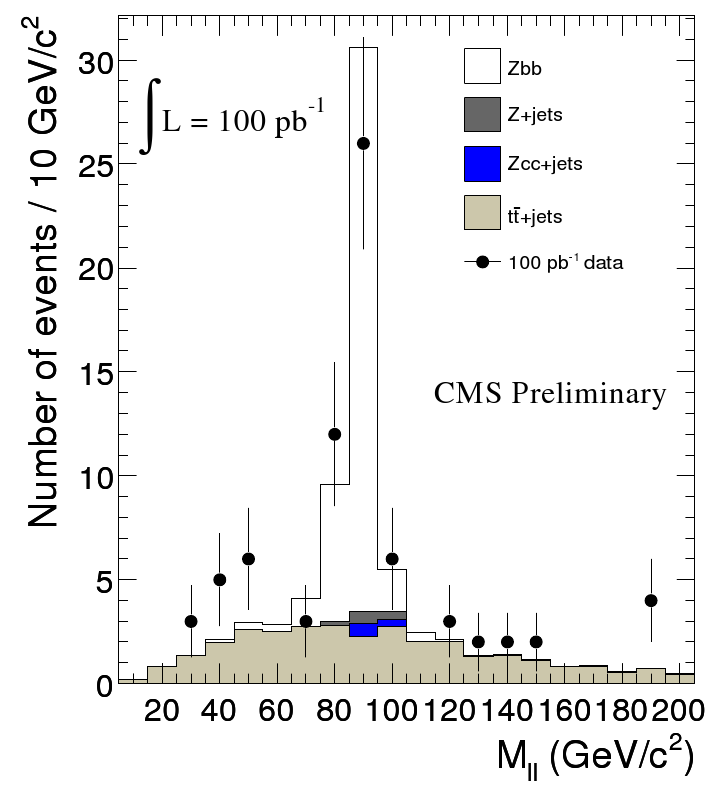
\includegraphics[width=0.95\linewidth]{Zbb_100pb-1.png}
\end{columns}

\vspace{-0.8 cm}
\begin{columns}
\column{0.3\linewidth}
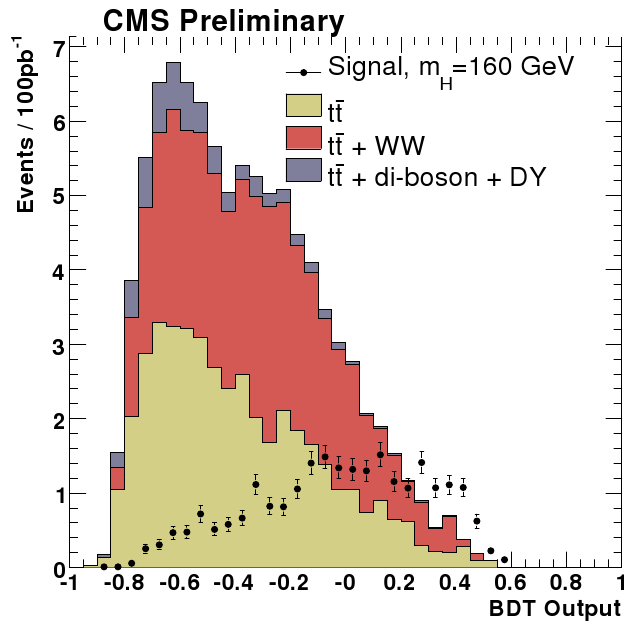
\includegraphics[width=1.333\linewidth]{Higgs_WW_100pb-1.png}

\column{0.6\linewidth}

\mbox{ }

\begin{itemize}
\item Higgs boson?  Even a heavy Higgs?
\begin{itemize}\setlength{\itemsep}{0.1 cm}
\item $H \to ZZ$ sensitivity \mbox{starts at 3~fb$^{-1}$\hspace{-1 cm}} \\ \mbox{\scriptsize (for 95\% C.L. in 200 $<$ $M_H$ $<$ 400~GeV)\hspace{-1 cm}}
\item $H \to WW$ has $\sim$10 signal, $\sim$10 background events at 100~pb$^{-1}$ with a \mbox{boosted decision tree analysis\hspace{-1 cm}}
\item comparable to Tevatron's reach
\end{itemize}
\end{itemize}
\end{columns}
%% 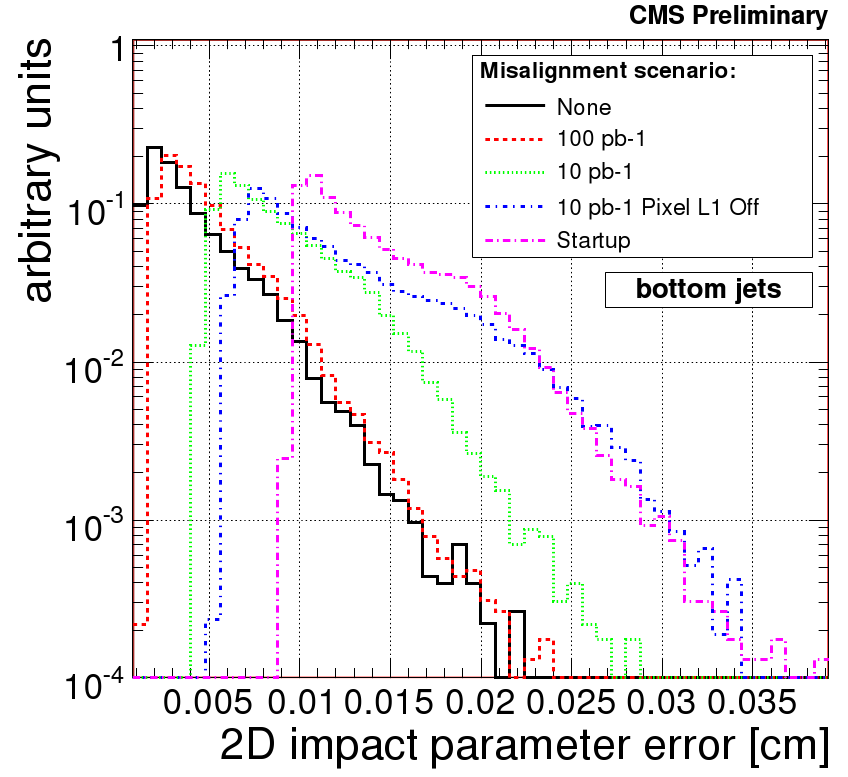
\includegraphics[width=0.25\linewidth]{btagging_error_vsmisalignment.png}
%% 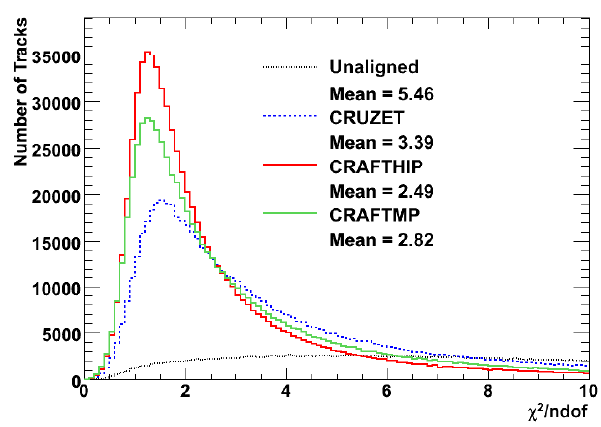
\includegraphics[width=0.25\linewidth]{tracker_alignment.png}
\label{discoveries_in_standard_model}
\end{frame}

\begin{frame}
\frametitle{SUSY at 100~pb$^{-1}$ (briefly)}
\begin{center}
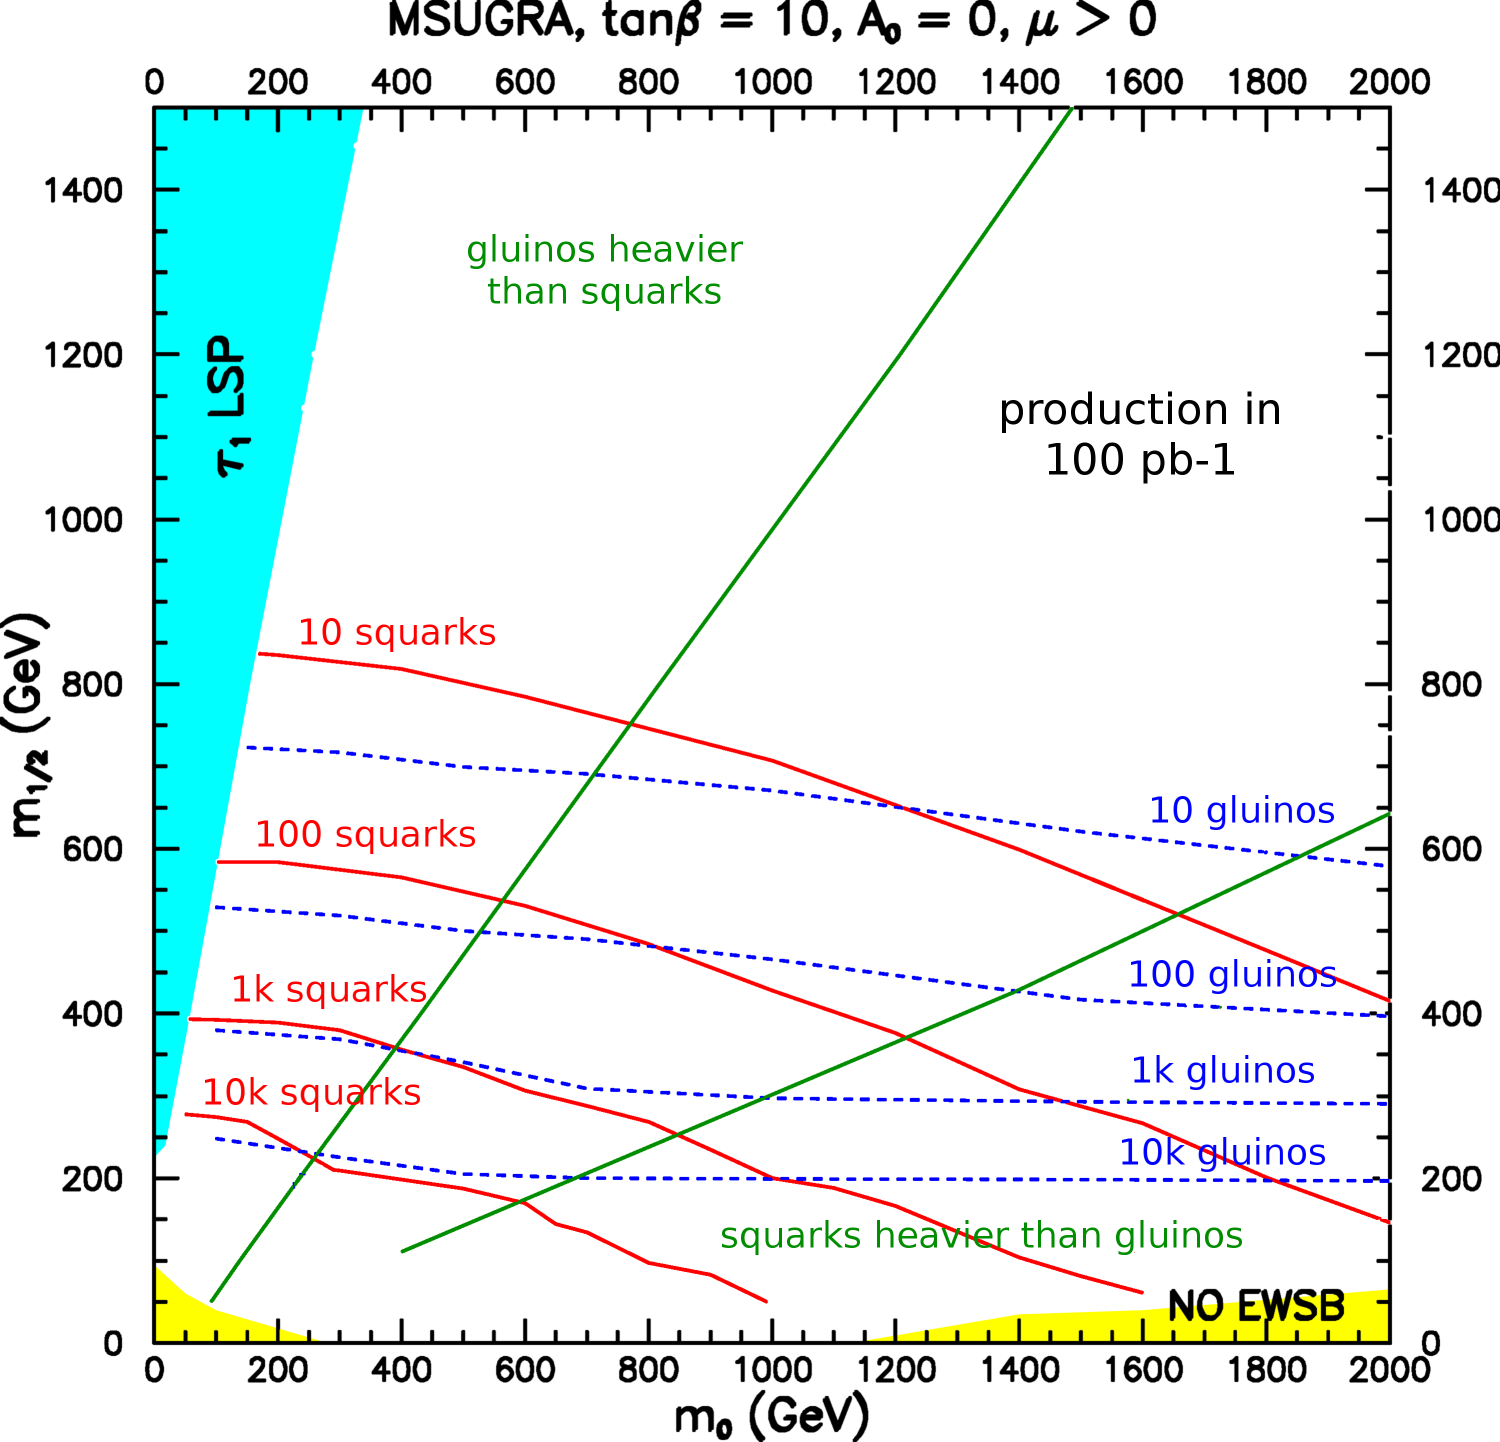
\includegraphics[width=0.65\linewidth]{msugra_plane_ptdr.png}
\end{center}

\vspace{-0.5 cm}
\begin{itemize}
\item From the Physics TDR (which focuses on 1~fb$^{-1}$ and above)
\item See Oliver and Anwar's talks for more details on SUSY modes
\end{itemize}
\label{susy_at_100ipb}
\end{frame}

%% \begin{frame}
%% \frametitle{100~pb$^{-1}$ example: SUSY in dijets}
%% \begin{itemize}
%% \item Background dijets from QCD are back-to-back and equal magnitude in the transverse plane
%% \item Dijets from SUSY $\tilde{q}\tilde{q} \to q\chi^0_1 \, q\chi^0_1$ are less correlated
%% \item Discriminating variables {\scriptsize (L.\ Randall and D.\ Tucker-Smith {\it arXiv:0806.1049})}:

%% \mbox{ } \hfill $\alpha = E_T(\mbox{jet 2}) / M_{\mbox{\scriptsize inv}}(\mbox{jets 1\&2})$ \hfill \mbox{ }

%% \mbox{ } \hfill $\alpha_T = E_T(\mbox{jet 2}) / M_{\mbox{\scriptsize transverse inv}}(\mbox{jets 1\&2})$ \hfill \mbox{ }

%% \item Example LM1: \mbox{$m_0=60$, $m_{1/2}=250$~GeV, $A_0=0$, $\tan\beta=10$, $\mu>0$\hspace{-1 cm}}
%% \end{itemize}

%% 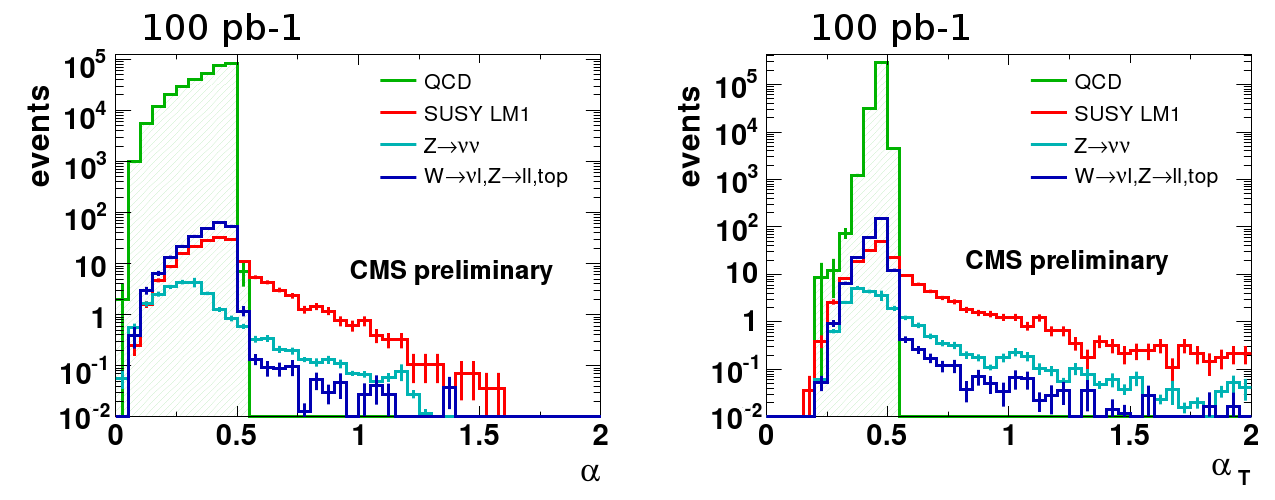
\includegraphics[width=\linewidth]{susy_dijet_angles.png}
%% \end{frame}

\begin{frame}
\frametitle{Di-object signature searches}

\begin{itemize}\setlength{\itemsep}{0.3 cm}
\item Look for a (high) mass peak or enhancement in inclusive $X$-$Y$ pairs,
  where $X$ and $Y$ are reconstructed ``physics objects'' like $e^\pm$, jet, \met

\item Between a specific-model hunt and completely generic search
\begin{itemize}\setlength{\itemsep}{0.1 cm}
\item physics motivation is strong but loosely-specified:
\begin{itemize}\setlength{\itemsep}{0.1 cm}
\item<1-| alert@1> \textcolor{darkblue}{di-muon:} \textcolor{black}{electroweak couples to leptons, easiest to identify}
\item<1-| alert@1> \textcolor{darkblue}{di-electron:} \textcolor{black}{electroweak couples to leptons, high-resolution calorimetry at high energy}
\item<1-| alert@1> \textcolor{darkblue}{di-jets:} \textcolor{black}{new physics may be strongly interacting,} \mbox{\textcolor{black}{high statistics}\hspace{-1 cm}}
\item<1-| alert@1> \textcolor{darkblue}{jet-\met:} \textcolor{black}{dark matter shows up as missing energy}
\item \textcolor{darkblue}{$t\bar{t}$:} new physics will likely be coupled to the third generation

\mbox{\scriptsize \it (demands new techniques because $W$ and $b$ jets overlap in boosted tops)\hspace{-1 cm}}
\item \textcolor{darkblue}{di-tau:} new physics will likely be coupled to \mbox{the third generation\hspace{-1 cm}}
\item \textcolor{darkblue}{$\gamma\gamma$:} easy way to identify spin-2 parent
\end{itemize}

%% \vspace{-0.3 cm}
%% \hfill {\scriptsize \textcolor{red}{$^*$}covered in this talk}

\item small set of simply defined channels (good for low statistics)
\end{itemize}

\item Also help to commission the reconstruction of physics objects
  for more sophisticated analyses
\end{itemize}
\end{frame}

\begin{frame}
\frametitle{Di-electrons/muons: $Z'$, RS-1 $G^*$}

\begin{columns}
\column{0.7\linewidth}

\begin{tabular}{c c}
$Z'_\psi \to e^+e^-$ & $Z'_\psi \to \mu^+\mu^-$ \\
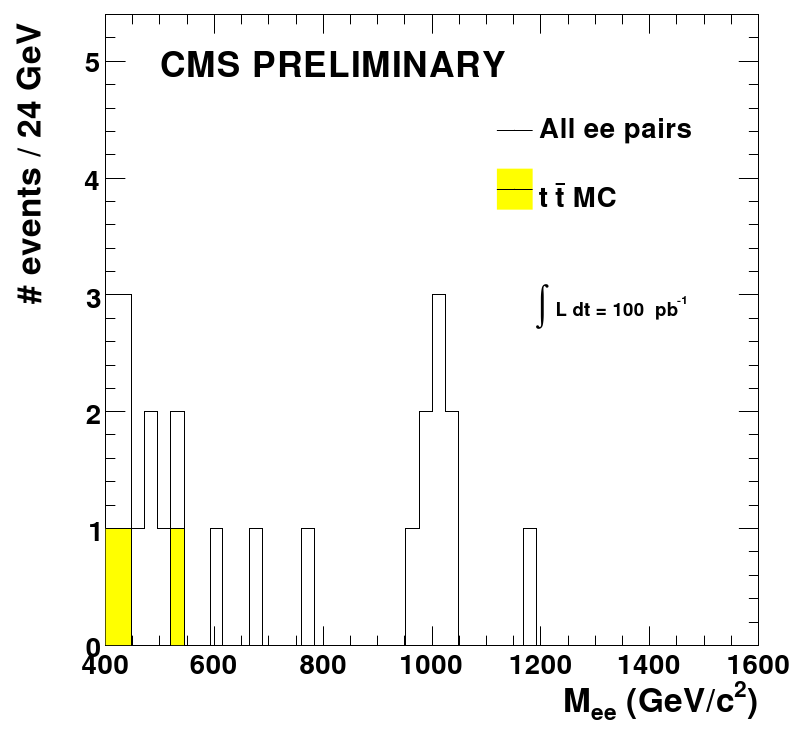
\includegraphics[height=3.5 cm]{Zpsi_ee_100pb-1.png} & 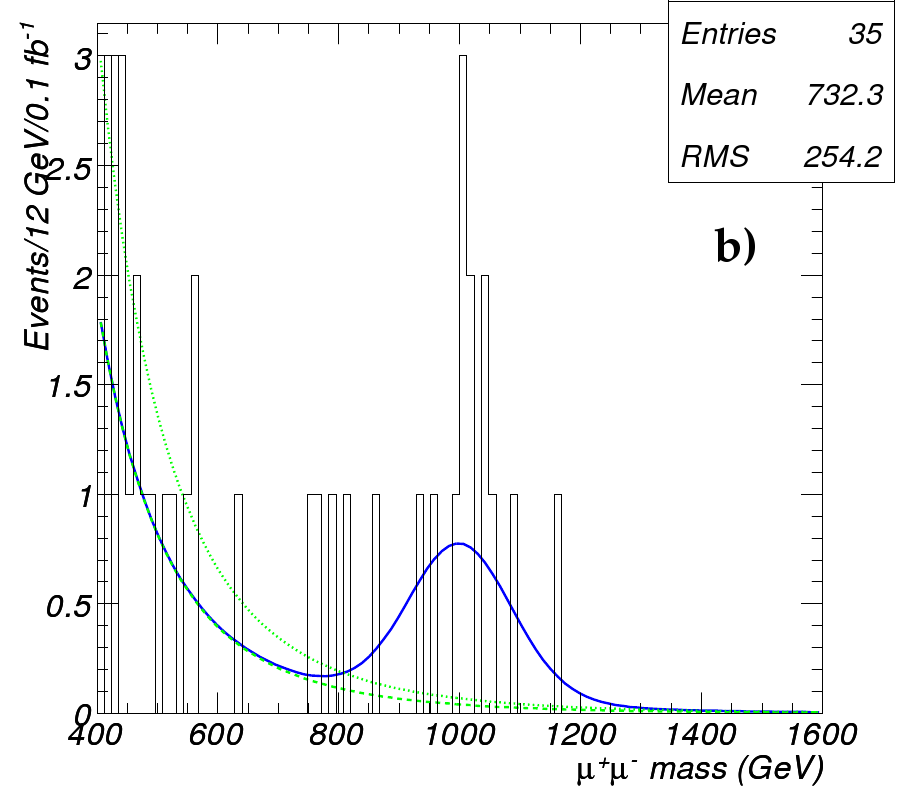
\includegraphics[height=3.5 cm]{Zpsi_mumu_100pb-1.png} \\

& \\

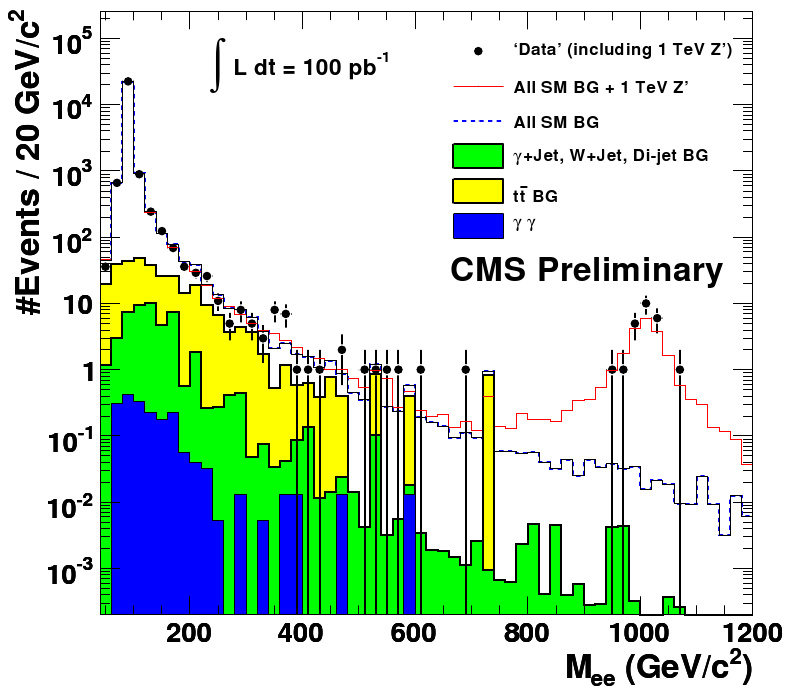
\includegraphics[height=3.5 cm]{Zprime_ee_backgrounds.png} & 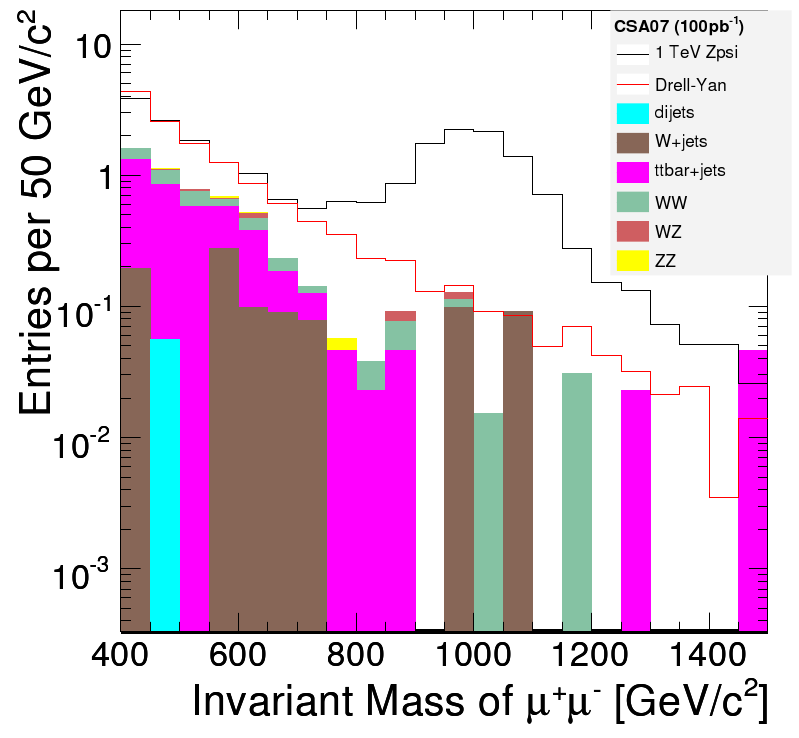
\includegraphics[height=3.5 cm]{Zprime_mumu_backgrounds.png} \\
\end{tabular}

\column{0.01\linewidth}

\column{0.35\linewidth}
\begin{itemize}\setlength{\itemsep}{0.25 cm}
\item Easiest-to-identify signature of new self-adjoint bosons (and therefore a very early analysis)

\item Long lever arm in muon tracking system helps to resolve straight tracks and high redundancy helps to distinguish delta rays from TeV muon showering
\end{itemize}
\end{columns}
\label{dielectrons_dimuons}
\end{frame}

\begin{frame}
\frametitle{Di-electrons/muons: $Z'$, RS-1 $G^*$}

\begin{itemize}
\item Measuring cross-section relative to $Z^0$ reduces \mbox{systematic uncertainties:\hspace{-1 cm}}
\begin{itemize}
\item integrated luminosity will only be known to 10--20\% in \mbox{early data\hspace{-1 cm}}
\item PDF uncertainties from $q\bar{q}$ initial states are reduced \mbox{in the ratio\hspace{-1 cm}}
\end{itemize}
\end{itemize}

\vfill
\mbox{ } \hfill \hfill \hfill absolute PDF uncertainty \hspace{1 cm} PDF uncertainty relative to $Z^0$ \hfill \mbox{ }

\mbox{ } \hfill 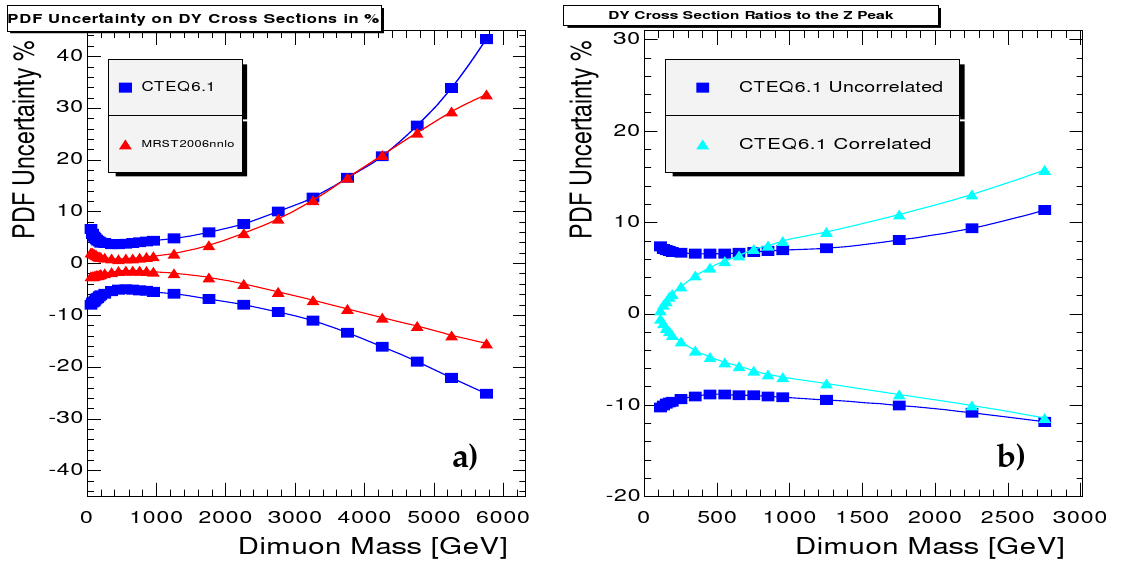
\includegraphics[width=0.9\linewidth]{Zprime_mumu_pdfuncert.png} \hfill \mbox{ }

\begin{itemize}
\item 95\% C.L.\ upper limit on an unobserved $Z_\psi$ cross-section \\ \hfill $\approx \left( \mbox{10--30} \times 10^{-6} \right) \times$ $Z^0$ cross-section
\end{itemize}

%% 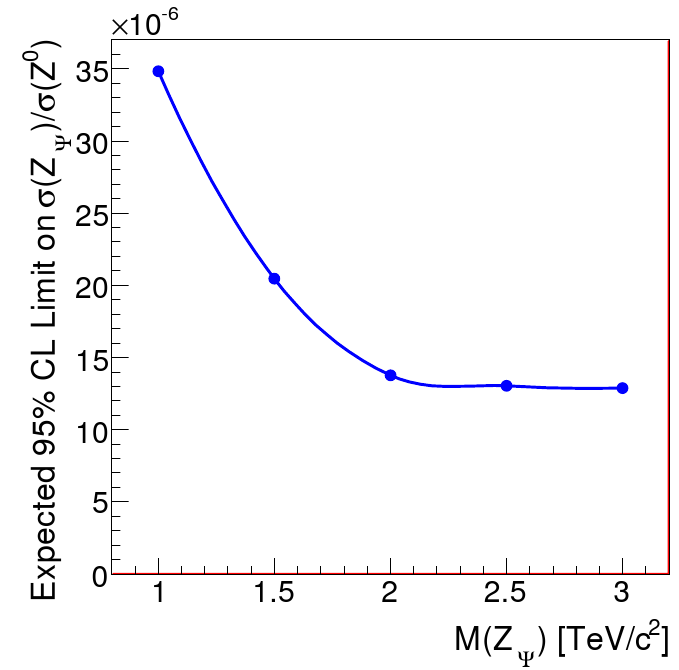
\includegraphics[height=3.8 cm]{Zprime_mumu_upperlimit.png}

%% \begin{columns}
%% \column{0.35\linewidth}

%% \begin{itemize}
%% \item 
%% \end{itemize}

%% \column{0.65\linewidth}
%% 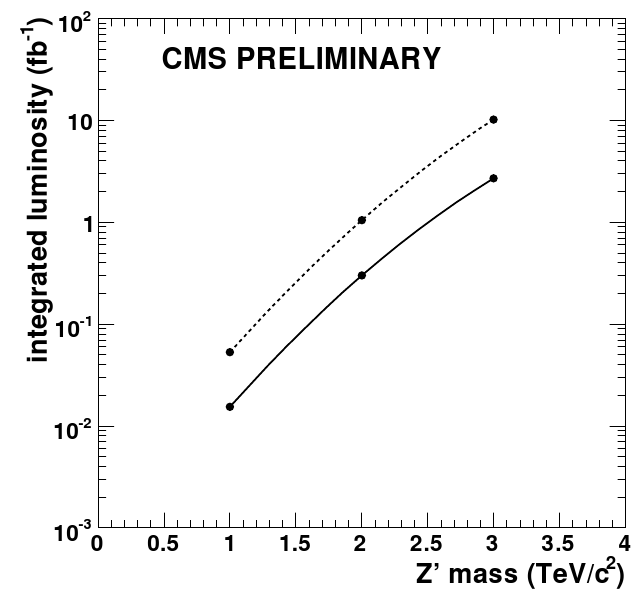
\includegraphics[height=2.8 cm]{Zprime_ee_limit_5sigma.png}
%% 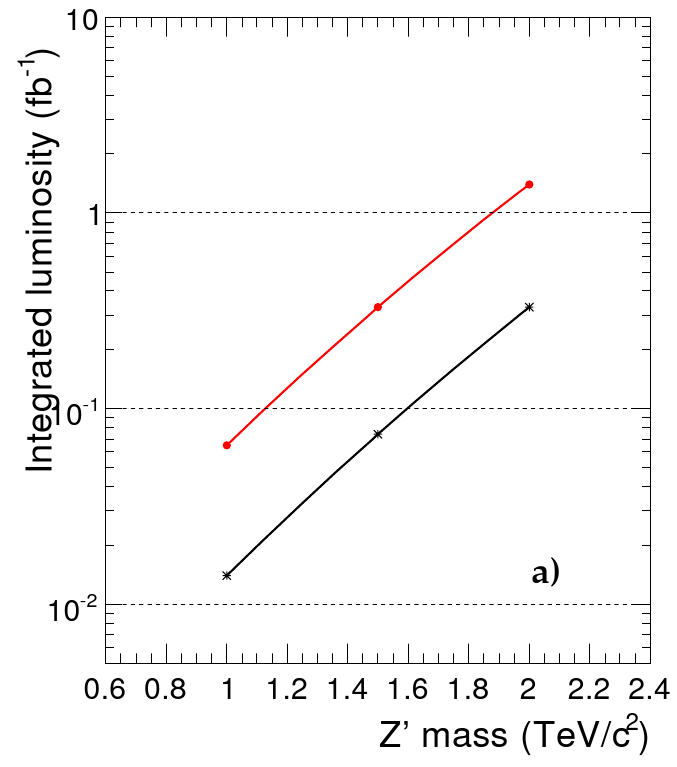
\includegraphics[height=2.8 cm]{Zprime_mm_limit_5sigma.png}
%% \end{columns}
%% 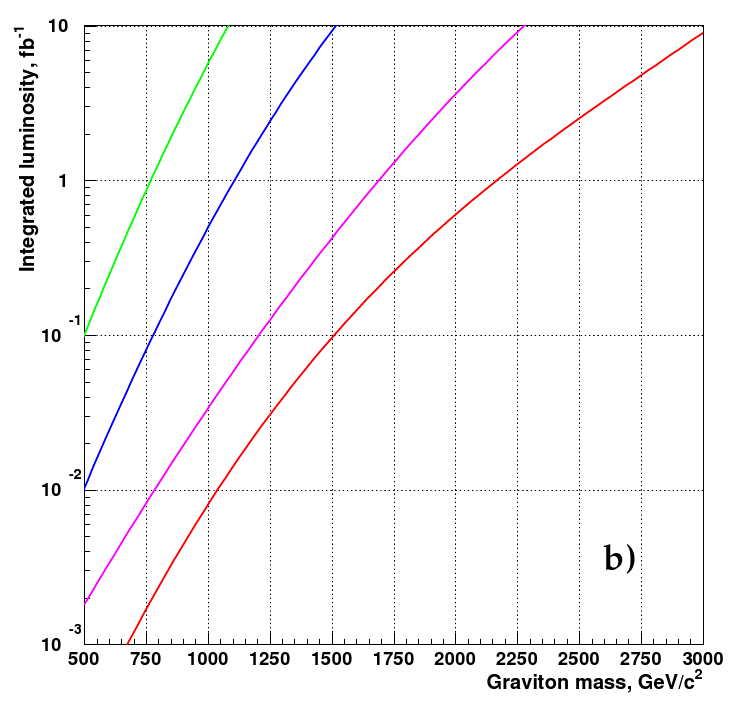
\includegraphics[width=0.25\linewidth]{RSG_mm_limit_5sigma.png}
\label{diobject_reach}
\end{frame}

\begin{frame}
\frametitle{Di-jets: contact interactions, $q^*$\hspace{-0.21 cm}, \hspace{0.1 cm}SUSY}

\vfill
\begin{columns}
\column{0.65\linewidth}
\begin{itemize}
\item Enhanced production at high mass \\ (for central $|\eta|$): \mbox{contact interactions\hspace{-1 cm}}

\item Resonance peaks: excited quarks ($q^*$), new bosons $Z'$, RS-1 $G^*$

\item Angular correlation: direct-decay SUSY e.g.\ $\tilde{q}\tilde{q} \to q\chi^0_1 \, q\chi^0_1$
\end{itemize}

\vspace{0.2 cm}
\mbox{ } \hfill 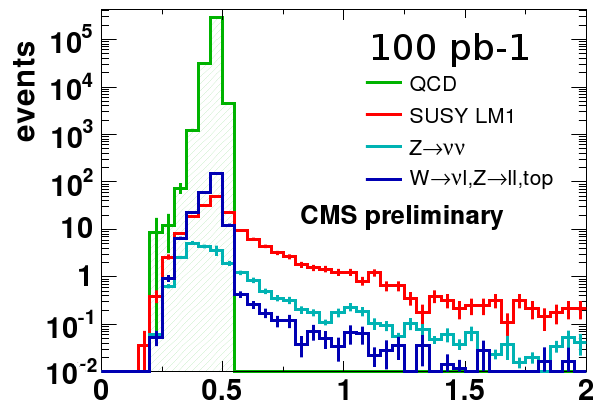
\includegraphics[width=0.75\linewidth]{susy_dijet_angles_transverse.png} \hfill \mbox{ }

\mbox{ } \hfill \hfill {\scriptsize $\alpha_T = E_T(\mbox{jet 2}) / M_{\mbox{\scriptsize transverse inv}}(\mbox{jets 1\&2})$} \hfill \mbox{ }

\mbox{ } \hfill \hfill {\scriptsize (L.\ Randall and D.\ Tucker-Smith \textcolor{blue}{\href{http://arxiv.org/abs/0806.1049}{arXiv:0806.1049}})} \hfill \mbox{ }

\column{0.43\linewidth}
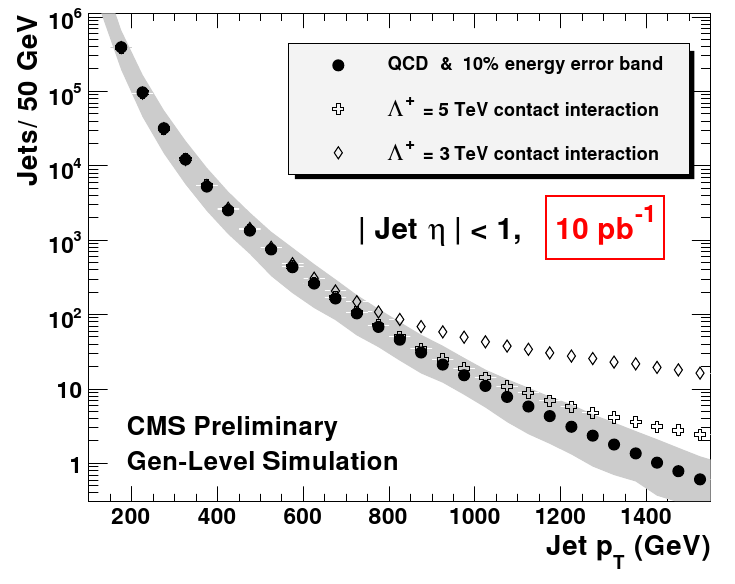
\includegraphics[width=\linewidth]{dijet_contactinteractions.png}

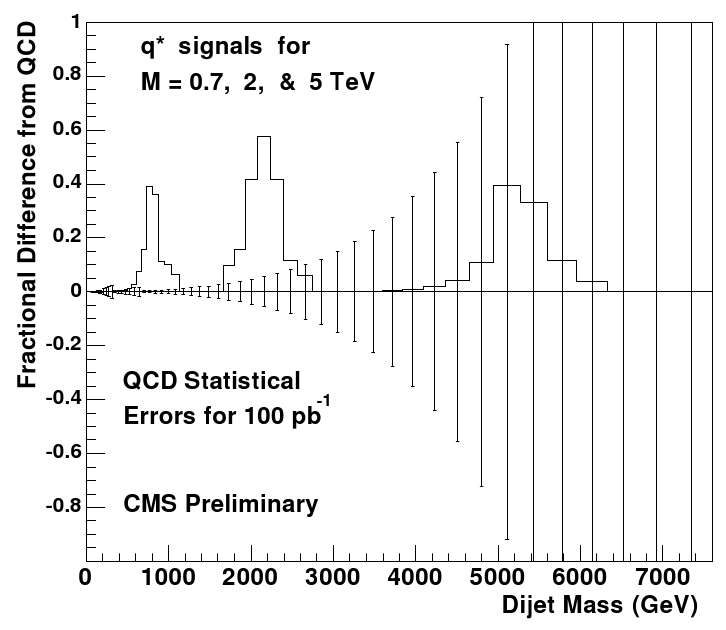
\includegraphics[width=\linewidth]{dijet_excited_quark.png}
\end{columns}
\label{dijets}
\end{frame}

\begin{frame}
\frametitle{\met $+$ 1 or more jets: ADD gravitons}
\begin{columns}
\column{0.7\linewidth}
\begin{itemize}
\item Simple signature: \met\ $+$ 1 jet is the missing energy analogue of a di-object search

\item Application: if extra dimensions lower the Plank mass to the TeV scale, real
  gravitons would be emitted in quark/gluon collisions \\ (ADD model and variations)

\item Optimistic case in 100~pb$^{-1}$ pictured below: \\ number of dimensions $\delta$ = 2 \\ compactification scale $M_D$ = 2~TeV

%% $M_D$ limits on ADD extra dimensions
%% {\scriptsize
%% \begin{tabular}{c c c c c}
%%  & 1 & 2 & 3 & 4 \\\hline
%% CDF & & 1.18 & 0.99 & 0.91 \\
%% D\O & & 0.99 & 0.80 & 0.73 \\
%% SN cooling & 30 & 2.5 & & \\
%% SN photon emission & 80 & 7 & & \\
%% Neutron star halo & 450 & 30 & & \\
%% \end{tabular}}
\end{itemize}

\vfill
\column{0.3\linewidth}

\scriptsize Significance in 100~pb$^{-1}$

\hspace{0.25 cm} 3 is 99.6\% C.L.

\hspace{0.25 cm} 5 is a 5$\sigma$ discovery

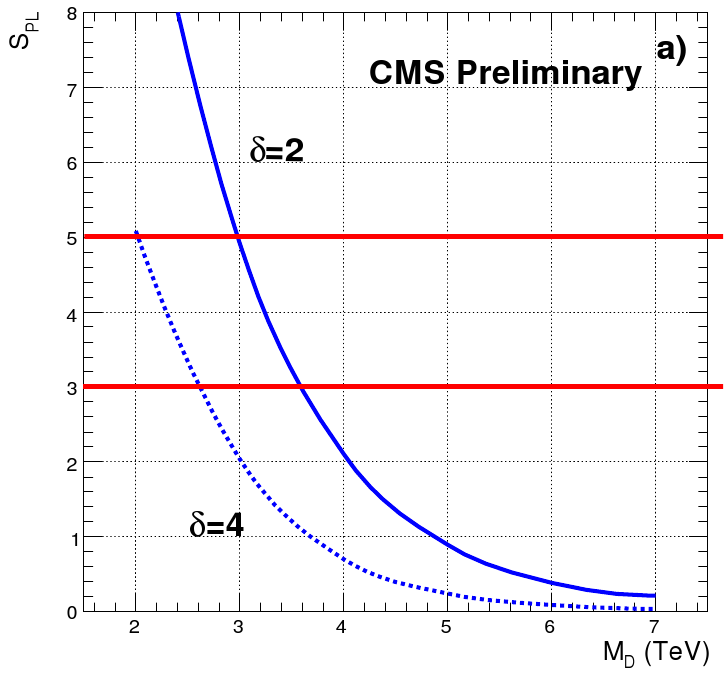
\includegraphics[width=\linewidth]{add_reach_100pb-1.png}
\end{columns}

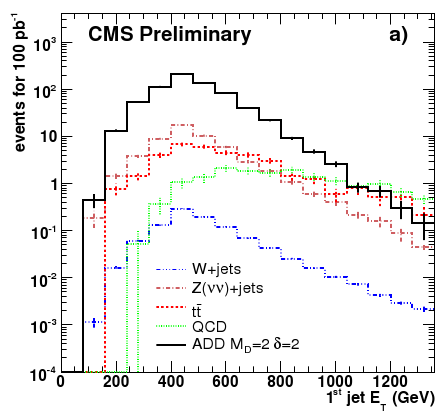
\includegraphics[width=0.35\linewidth]{add_jet1_100pb-1.png}
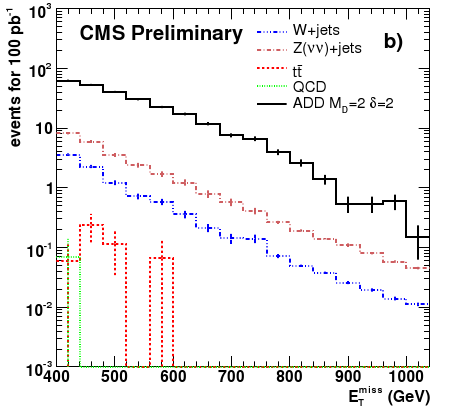
\includegraphics[width=0.35\linewidth]{add_met_100pb-1.png}
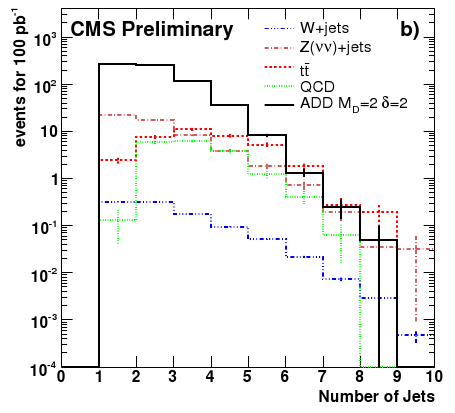
\includegraphics[width=0.35\linewidth]{add_njets_100pb-1.png}
\label{onejet_onemet}
\end{frame}

\begin{frame}
\frametitle{\met\ commissioning \textcolor{gray}{(optional slide)}}

\vfill
\begin{columns}
\column{0.6\linewidth}

\begin{itemize}\setlength{\itemsep}{0.15 cm}
\item Missing energy is a physics object commissioned in simple signatures, to be used later in dark matter searches

\item Decomposition of \met\ resolution \mbox{(top plot)\hspace{-1 cm}}

\mbox{\scriptsize $\sigma(\mbox{\met}) = \textcolor{darkblue}{A} \oplus \textcolor{darkblue}{B} \sqrt{\sum\mbox{\met} - \textcolor{darkblue}{D}} \oplus \textcolor{darkblue}{C} (\sum\mbox{\met} - \textcolor{darkblue}{D})$ \hspace{-1 cm}}

\renewcommand\theenumi{\Alph{enumi}}
\begin{enumerate} \scriptsize
\item \scriptsize electronic noise, pile-up, \mbox{underlying event\hspace{-1 cm}}
\item \scriptsize statistical sampling in \mbox{calorimeter towers\hspace{-1 cm}}
\item \scriptsize non-linearities, cracks, \mbox{dead material\hspace{-1 cm}}
\item \scriptsize effect of noise, etc.\ on $\sum$\met
\end{enumerate}

{\scriptsize where \met\ $=$ $\left|\mbox{vector missing momentum}\right|$ \\ and $\sum$\met\ $=$ the scalar sum}

\item Snapshot from real data: response of calorimeter towers to muons, a \met\ correction, as seen in cosmic rays (bottom plot)

\item \textcolor{darkblue}{See James Lamb and Paolo Rumerio's talks for more}
\end{itemize}

\vspace{0.25 cm}

\column{0.43\linewidth}
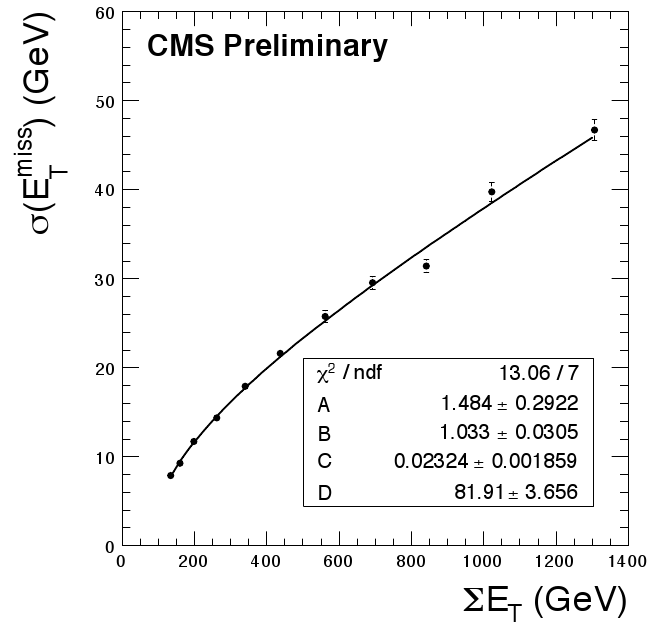
\includegraphics[width=\linewidth]{missing_energy_resolution.png}

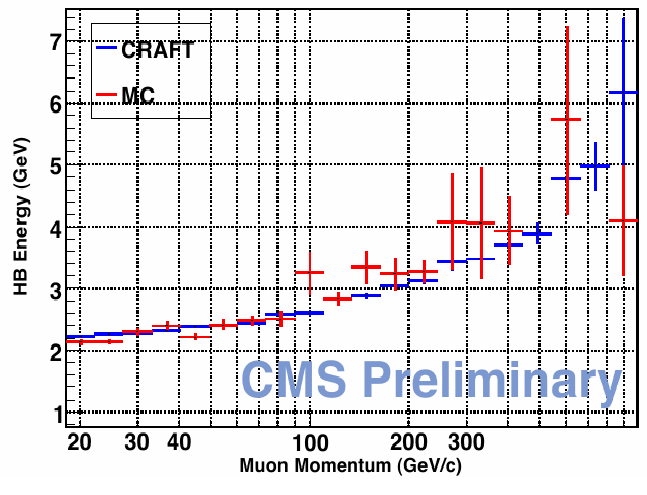
\includegraphics[width=\linewidth]{HCAL_muon_response.png}

% 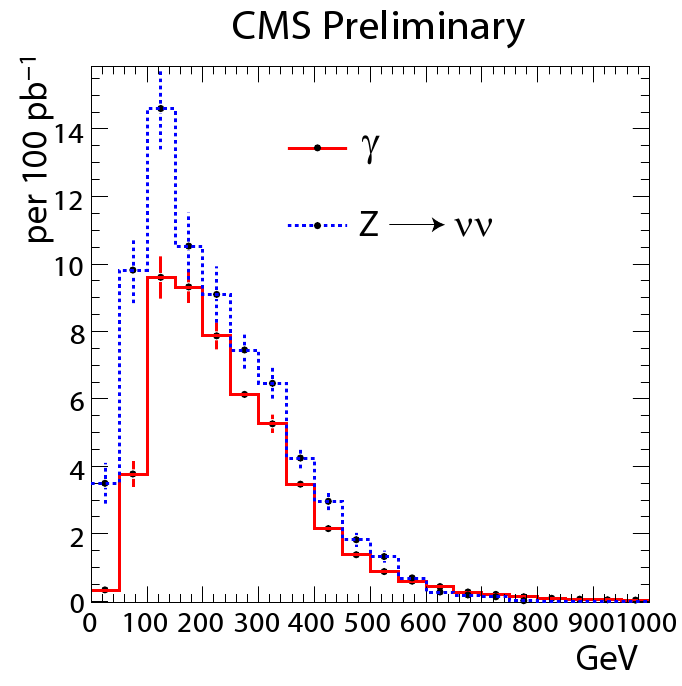
\includegraphics[width=\linewidth]{Z_nunu_estimation_with_photon.png}

\end{columns}
% 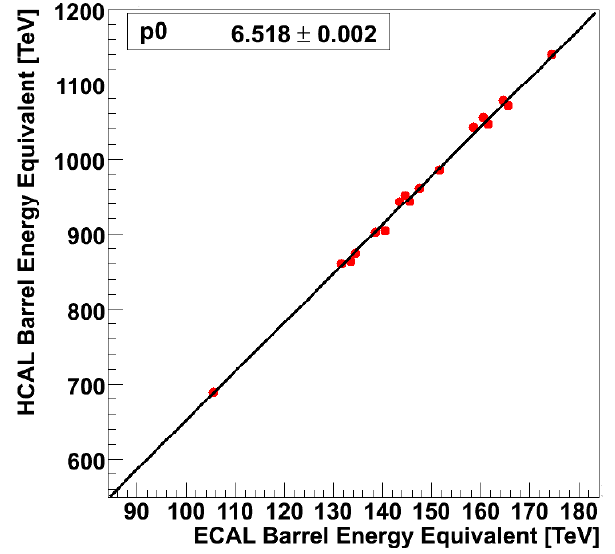
\includegraphics[width=0.25\linewidth]{ECAL-HCAL_correlation.png}
\label{missing_energy}
\end{frame}

\begin{frame}
\frametitle{Heavy, long-lived charged particles}

\begin{columns}
\column{0.6\linewidth}
\begin{itemize}
\item New particles might be charged and live long enough to be detected \\ (split SUSY, part of WIMP sector\ldots)

\item Unusual detector signature: would look like a muon with the
  wrong timing in the CMS drift tubes \mbox{(top figure)\hspace{-0.5 cm}} and low-velocity \mbox{$dE/dx$ in silicon tracker\hspace{-3 cm}}

\item Requiring a correlation yields \mbox{low backgrounds at high mass:\hspace{-4 cm}} 500~GeV stop from split SUSY \mbox{with 100~pb$^{-1}$ shown at bottom-right\hspace{-5 cm}}

\end{itemize}

\column{0.4\linewidth}
\hfill 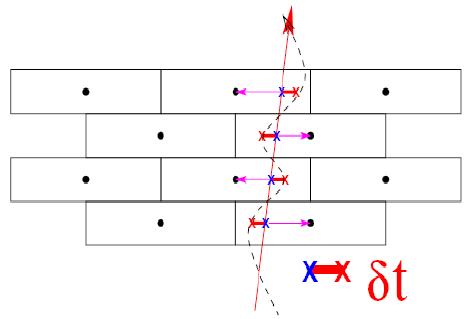
\includegraphics[width=\linewidth]{champ_track_signature.png}
% 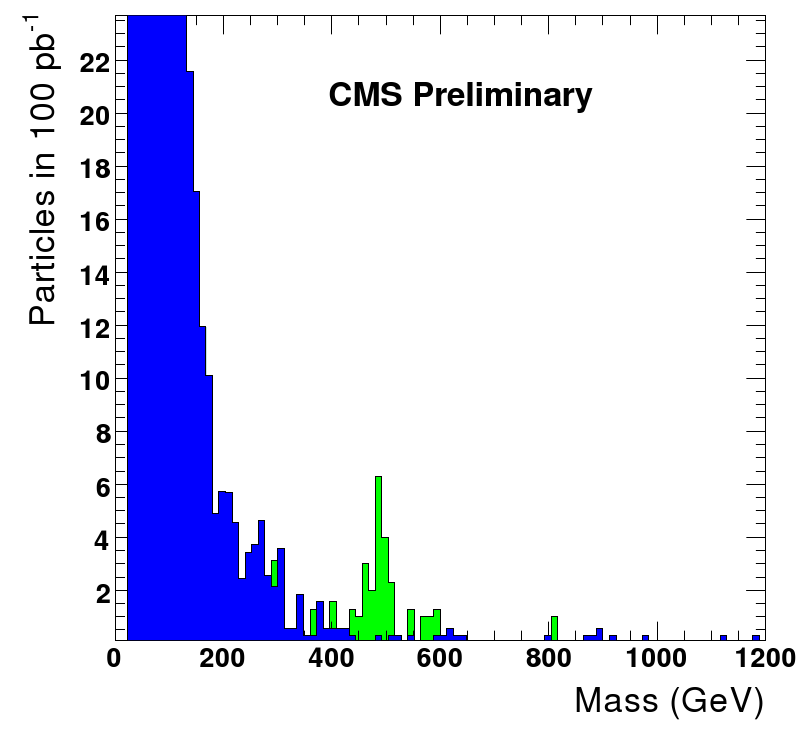
\includegraphics[width=\linewidth]{champ_backgrounds.png}

\vspace{0.5 cm}
\mbox{ }
\end{columns}

\vspace{0.15 cm}
\begin{columns}
\column{0.7\linewidth}
\scriptsize \mbox{ } \hspace{1 cm} background \hspace{1 cm} \hfill signal \hfill \mbox{ }
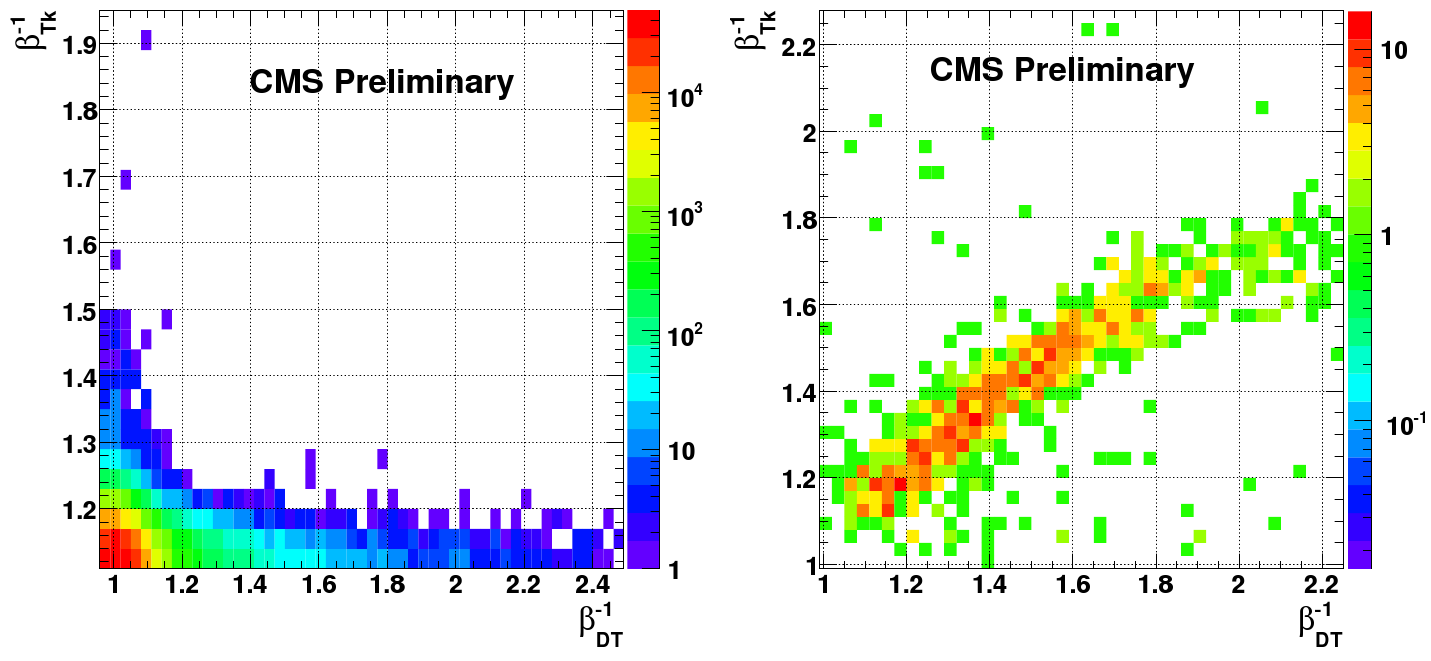
\includegraphics[width=\linewidth]{champ_invbeta.png}

\column{0.4\linewidth}
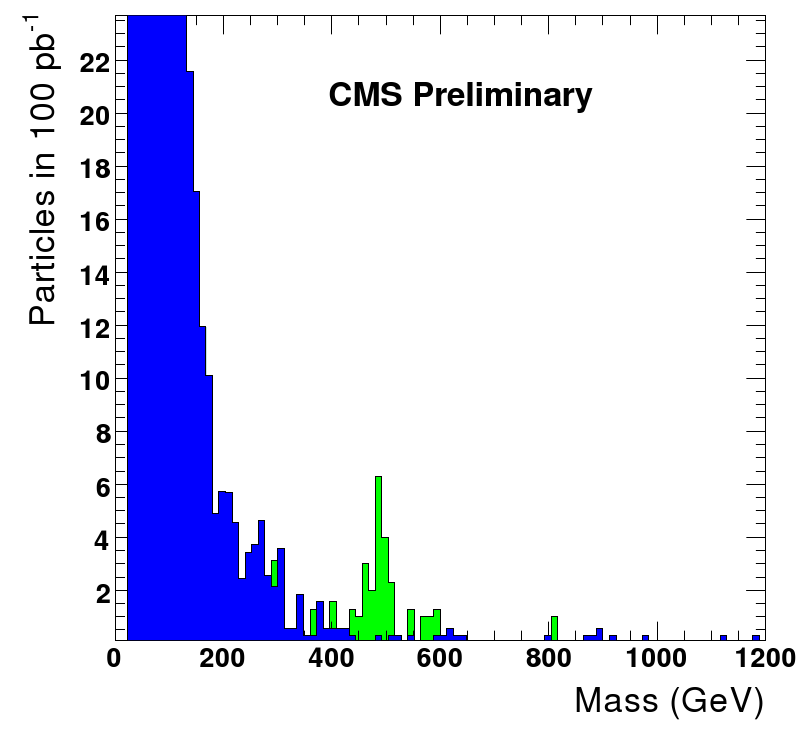
\includegraphics[width=\linewidth]{champ_backgrounds.png}

%% \mbox{ } \hfill \hspace{0.4 cm} discovery \hspace{2.0 cm} exclusion \hfill \mbox{ }

%% 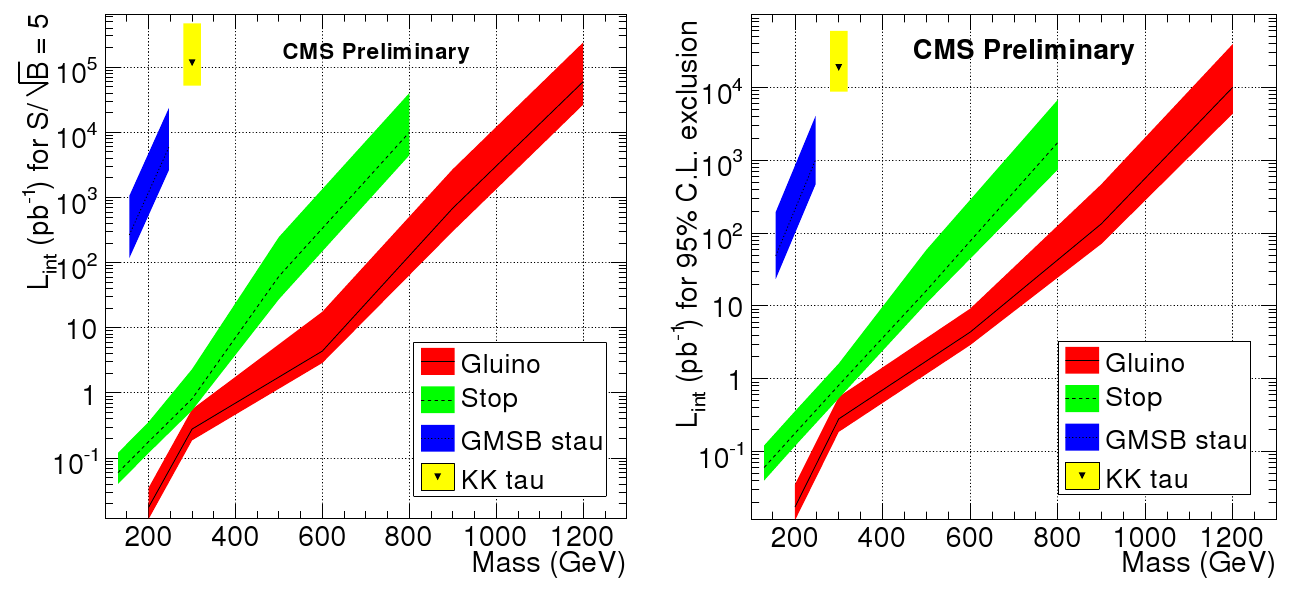
\includegraphics[width=\linewidth]{champ_reach.png}
\end{columns}
\label{champs}
\end{frame}

%% \begin{frame}
%% \frametitle{Generic, model-independent search}

%% 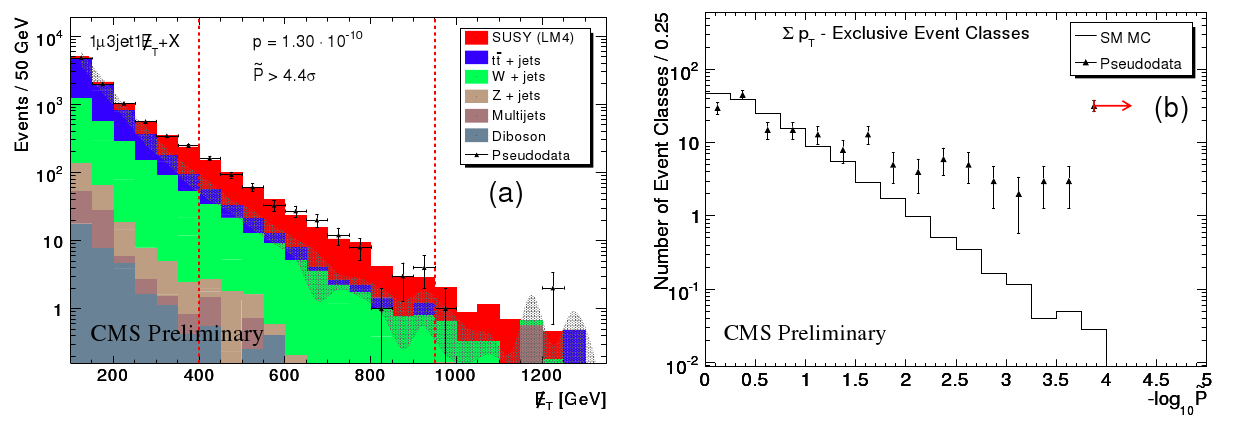
\includegraphics[width=\linewidth]{music.png}
%% \end{frame}

\begin{frame}
\frametitle{Other new results}

\vspace{-0.4 cm}
\begin{columns}
\column{0.45\linewidth}
\begin{itemize}
\item $W' \to e \nu$ (plot at right)
\begin{itemize}
\item enlarged gauge groups usually predict a new $W'$ as well as $Z'$
\item can also be thought of as an $e+$\met\ di-object search
\end{itemize}
\end{itemize}

\mbox{ }

\column{0.65\linewidth}

\vspace{0.5 cm}
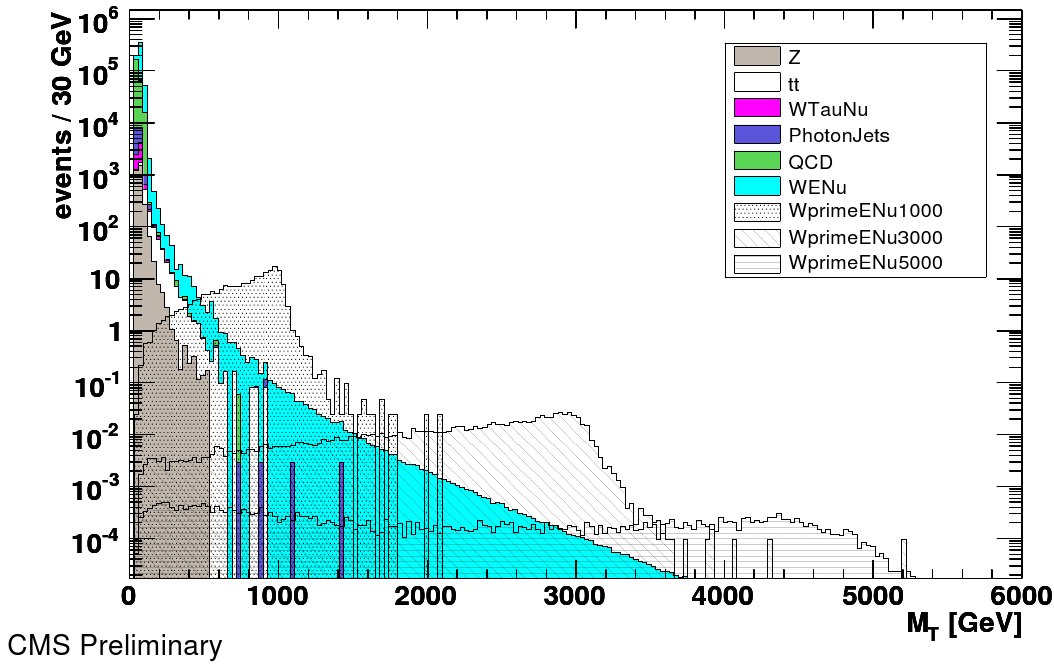
\includegraphics[width=\linewidth]{Wprime_enu_backgrounds.png}
\end{columns}

\vspace{-1.3 cm}
\begin{columns}
\column{1.13\linewidth}
\begin{itemize}
\item $b'b' \to WWWW \, bb$
\begin{itemize}
\item 1--4 leptons $+$ 2 $b$-jets
\item 100~pb$^{-1}$ 95\% exclusion at the few-pb level up to $M_{b'}$ = 480~GeV \\ (well below predicted cross-section for these masses)
\end{itemize}

\item Heavy Majorana neutrino $\to \ell W_R$ with $W_R \to$ jet jet
\begin{itemize}
\item signature 1: dijet mass peak $+$ 2 leptons (produced through $W_R$)
\item signature 2: dijet mass peak $+$ 1 lepton (produced through $Z_R$)
\end{itemize}

\item Model Unspecific Search in CMS (MUSiC)
\begin{itemize}
\item 300--400 combinations of $e$, $\mu$, $\gamma$, jet, \met
\end{itemize}

\end{itemize}
\end{columns}
\label{others}
\end{frame}

%% \begin{frame}
%% \frametitle{$W' \to \ell\nu$}

%% 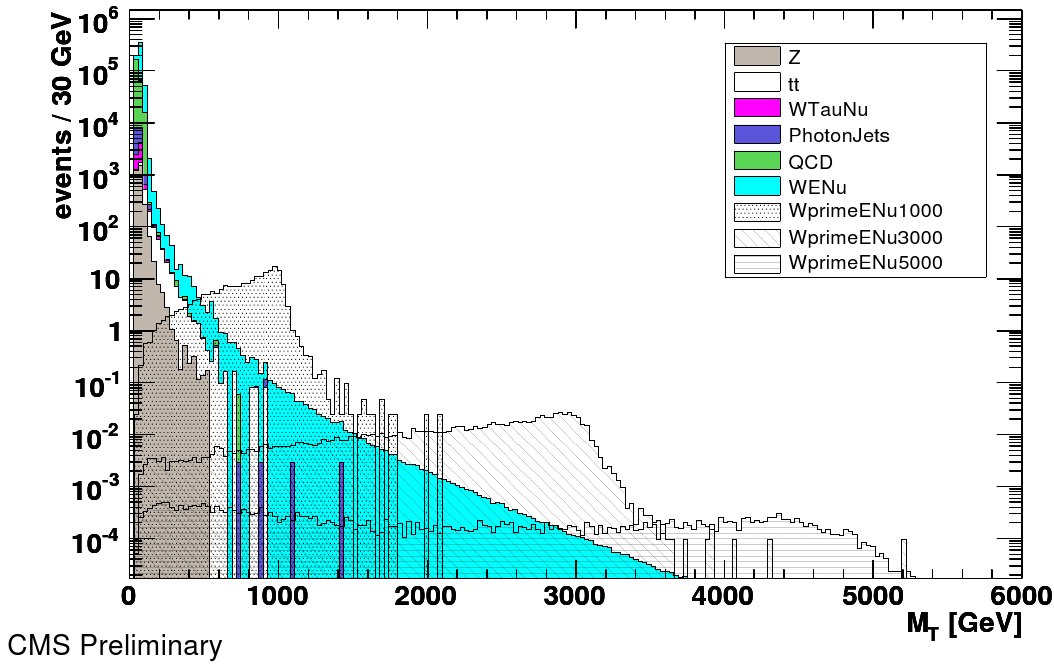
\includegraphics[width=0.25\linewidth]{Wprime_enu_backgrounds.png}
%% \includegraphics[width=0.25\linewidth]{Wprime_enu_triggereff.png}

%% \end{frame}

%% \begin{frame}
%% \frametitle{$b' \to WWWW$}

%% \includegraphics[width=0.25\linewidth]{bprime_WWWW.png}

%% \end{frame}

\begin{frame}
\frametitle{Conclusions}

\begin{itemize}\setlength{\itemsep}{0.5 cm}
\item With 100~pb$^{-1}$, we can do more than \mbox{``rediscover the Standard Model''\hspace{-1 cm}}

\item Di-object searches are a simple way to address broad classes of
  new physics with small statistics, and at the same time improve our
  understanding of the detector response

\item Understanding the detector with real data will be key to all
  analyses, early and long-term

\item Trigger and pattern recognition are also being made sensitive to
  unusual detector signatures like long-lived charged particles,
  $R$-hadrons that stop in the calorimeter or cavern, etc.

\item Not everything was included in this talk, I hoped to highlight
  those analyses which can be performed with low statistics
\end{itemize}

\label{numpages}
\end{frame}

%% \section*{First section}
%% \begin{frame}
%% \begin{center}
%% \Huge \textcolor{blue}{First section}
%% \end{center}
%% \end{frame}

\scriptsize

\begin{frame}
\frametitle{References (external hyperlinks)}

\vfill
\begin{columns}
\column{1.05\linewidth}
\renewcommand{\arraystretch}{1.04}
\begin{tabular}{c p{0.9\linewidth}}
Page & Reference \\\hline\hline
\pageref{rediscovering_standard_model} & \textcolor{blue}{\href{http://cms-physics.web.cern.ch/cms-physics/public/EWK-08-005-pas.pdf}{EWK-08-005}} {\it Measurement of the $W$ and $Z$ cross section with electrons} \\
 & \textcolor{blue}{\href{http://cms-physics.web.cern.ch/cms-physics/public/EWK-07-002-pas.pdf}{EWK-07-002}} {\it Measurement of the $W$ and $Z$ cross section with electrons} \\
\pageref{using_standard_model_for_future} & \textcolor{blue}{\href{http://cms-physics.web.cern.ch/cms-physics/public/EGM-07-001-pas.pdf}{EGM-07-001}} {\it Measuring Electron Efficiencies with Early Data} \\
 & \textcolor{blue}{\href{http://cms-physics.web.cern.ch/cms-physics/public/EWK-08-002-pas.pdf}{EWK-08-002}} {\it $W$ charge asymmetry} \\
\pageref{discoveries_in_standard_model} & \textcolor{blue}{\href{http://cms-physics.web.cern.ch/cms-physics/public/EWK-08-001-pas.pdf}{EWK-08-001}} {\it Measurement of $Z$ boson production in association with two $b$-jets} \\
 & From Figure 3.5 (page 54) \textcolor{blue}{\href{http://cdsweb.cern.ch/record/942733}{CMS-TDR-008-2}} {\it CMS Physics TDR: Vol.\ II} \\
 & \textcolor{blue}{\href{http://cms-physics.web.cern.ch/cms-physics/public/HIG-07-001-pas.pdf}{HIG-07-001}} {\it Higgs to $WW$} \\
\pageref{susy_at_100ipb} & Relabeling of \textcolor{blue}{\href{http://cdsweb.cern.ch/record/942733}{CMS-TDR-008-2}} Figure 13.1 (page 405) for 100~pb$^{-1}$ production \\
\pageref{dielectrons_dimuons} & \textcolor{blue}{\href{http://cms-physics.web.cern.ch/cms-physics/public/EXO-08-001-pas.pdf}{EXO-08-001}} {\it Search for $Z' \to ee$} \\
 & \textcolor{blue}{\href{http://cms-physics.web.cern.ch/cms-physics/public/SBM-07-002-pas.pdf}{SBM-07-002}} {\it Search for $Z' \to \mu\mu$} \\
\pageref{diobject_reach} & {\it Ibid.} \\
 & Pavel Nadolsky {\it CTEQ PDF developments} at \textcolor{blue}{\href{indico.cern.ch/conferenceDisplay.py?confId=27439}{PDF4LHC Workshop}}, Feb 22, 2008 \\
\pageref{dijets} & \textcolor{blue}{\href{http://cms-physics.web.cern.ch/cms-physics/public/SBM-07-001-pas.pdf}{SBM-07-001}} {\it Searches for New Physics using high ET dijet events} \\
 & \textcolor{blue}{\href{http://cms-physics.web.cern.ch/cms-physics/public/SUS-08-005-pas.pdf}{SUS-08-005}} {\it SUSY search with dijet events} (relabeled for 100~pb$^{-1}$) \\
\pageref{onejet_onemet} & \textcolor{blue}{\href{http://cms-physics.web.cern.ch/cms-physics/public/EXO-08-011-pas.pdf}{EXO-08-011}} {\it Search for extra dimensions with monojets} \\
\pageref{missing_energy} & \textcolor{blue}{\href{http://cms-physics.web.cern.ch/cms-physics/public/JME-07-001-pas.pdf}{JME-07-001}} {\it Performance of missing ET reconstruction} \\
 & \textcolor{blue}{\href{http://indico.cern.ch/conferenceDisplay.py?confId=43093}{Approved DPG Commissioning Results}} (internal CMS) \\
\pageref{champs} & \textcolor{blue}{\href{http://cms-physics.web.cern.ch/cms-physics/public/EXO-08-003-pas.pdf}{EXO-08-003}} {\it Search for Heavy Stable Charged Particles} \\
\pageref{others} & \textcolor{blue}{\href{http://cms-physics.web.cern.ch/cms-physics/public/EXO-08-004-pas.pdf}{EXO-08-004}} {\it Search for $W' \to e\nu$} \\
 & \textcolor{blue}{\href{http://cms-physics.web.cern.ch/cms-physics/public/EXO-08-009-pas.pdf}{EXO-08-009}} {\it Search for a $b'$} \\
 & \textcolor{blue}{\href{http://mkirsano.web.cern.ch/mkirsano/cmsanalysis/heavynu-cmsnote.pdf}{CMS NOTE 2006/098}} {\it Heavy Majorana $\nu$ and right-handed bosons} (internal CMS) \\
 & \textcolor{blue}{\href{http://cms-physics.web.cern.ch/cms-physics/public/EXO-08-005-pas.pdf}{EXO-08-005}} {\it MUSiC--- deviations between data and Monte Carlo simulation} \\\hline\hline
\end{tabular}
\end{columns}

\vfill
See \textcolor{blue}{\tt \href{https://twiki.cern.ch/twiki/bin/view/CMS/PhysicsResults}{https://twiki.cern.ch/twiki/bin/view/CMS/PhysicsResults}} for more
\end{frame}

\end{document}
